%%% Title presen0607
\documentclass[landscape,10pt]{ujarticle}
\special{papersize=\the\paperwidth,\the\paperheight}
\usepackage{ketpic,ketlayer}
\usepackage{ketslide}
\usepackage{amsmath,amssymb}
\usepackage{bm,enumerate}
\usepackage[dvipdfmx]{graphicx}
\usepackage{color}
\definecolor{slidecolora}{cmyk}{0.98,0.13,0,0.43}
\definecolor{slidecolorb}{cmyk}{0.2,0,0,0}
\definecolor{slidecolorc}{cmyk}{0.2,0,0,0}
\definecolor{slidecolord}{cmyk}{0.2,0,0,0}
\definecolor{slidecolore}{cmyk}{0,0,0,0.5}
\definecolor{slidecolorf}{cmyk}{0,0,0,0.5}
\definecolor{slidecolori}{cmyk}{0.98,0.13,0,0.43}
\def\setthin#1{\def\thin{#1}}
\setthin{0}
\newcommand{\slidepage}[1][s]{%
\setcounter{ketpicctra}{18}%
\if#1m \setcounter{ketpicctra}{1}\fi
\hypersetup{linkcolor=black}%

\begin{layer}{118}{0}
\putnotee{122}{-\theketpicctra.05}{\small\thepage/\pageref{pageend}}
\end{layer}\hypersetup{linkcolor=blue}

}
\usepackage{emath}
\usepackage{emathEy}
\usepackage{emathMw}
\usepackage{pict2e}
\usepackage{ketlayermorewith2e}
\usepackage[dvipdfmx,colorlinks=true,linkcolor=blue,filecolor=blue]{hyperref}
\newcommand{\hiduke}{0607}
\newcommand{\hako}[2][1]{\fbox{\raisebox{#1mm}{\mbox{}}\raisebox{-#1mm}{\mbox{}}\,\phantom{#2}\,}}
\newcommand{\hakoa}[2][1]{\fbox{\raisebox{#1mm}{\mbox{}}\raisebox{-#1mm}{\mbox{}}\,#2\,}}
\newcommand{\hakom}[2][1]{\hako[#1]{$#2$}}
\newcommand{\hakoma}[2][1]{\hakoa[#1]{$#2$}}
\def\rad{\;\mathrm{rad}}
\def\deg#1{#1^{\circ}}
\newcommand{\sbunsuu}[2]{\scalebox{0.6}{$\bunsuu{#1}{#2}$}}
\def\pow{$\hspace{-1.5mm}^\hspace{-1mm}$}
\def\dlim{\displaystyle\lim}
\newcommand{\brd}[2][1]{\scalebox{#1}{\color{red}\fbox{\color{black}$#2$}}}
\newcommand\down[1][0.5zw]{\vspace{#1}\\}
\newcommand{\sfrac}[3][0.65]{\scalebox{#1}{$\frac{#2}{#3}$}}
\newcommand{\phn}[1]{\phantom{#1}}
\newcommand{\scb}[2][0.6]{\scalebox{#1}{#2}}
\newcommand{\dsum}{\displaystyle\sum}

\setmargin{25}{145}{15}{100}

\ketslideinit

\pagestyle{empty}

\begin{document}

\begin{layer}{120}{0}
\putnotese{0}{0}{{\Large\bf
\color[cmyk]{1,1,0,0}

\begin{layer}{120}{0}
{\Huge \putnotes{60}{20}{インストール状況}}
\putnotes{60}{50}{高遠節夫}
\end{layer}

}
}
\end{layer}

\def\mainslidetitley{22}
\def\ketcletter{slidecolora}
\def\ketcbox{slidecolorb}
\def\ketdbox{slidecolorc}
\def\ketcframe{slidecolord}
\def\ketcshadow{slidecolore}
\def\ketdshadow{slidecolorf}
\def\slidetitlex{6}
\def\slidetitlesize{1.3}
\def\mketcletter{slidecolori}
\def\mketcbox{yellow}
\def\mketdbox{yellow}
\def\mketcframe{yellow}
\def\mslidetitlex{62}
\def\mslidetitlesize{2}

\color{black}
\Large\bf\boldmath
\addtocounter{page}{-1}

\def\MARU{}
\renewcommand{\MARU}[1]{{\ooalign{\hfil$#1$\/\hfil\crcr\raise.167ex\hbox{\mathhexbox20D}}}}
\renewcommand{\slidepage}[1][s]{%
\setcounter{ketpicctra}{18}%
\if#1m \setcounter{ketpicctra}{1}\fi
\hypersetup{linkcolor=black}%
\begin{layer}{118}{0}
\putnotee{115}{-\theketpicctra.05}{\small\hiduke-\thepage/\pageref{pageend}}
\end{layer}\hypersetup{linkcolor=blue}
}
\newcounter{ban}
\setcounter{ban}{1}
\newcommand{\monban}[1][\hiduke]{%
#1-\theban\ %
\addtocounter{ban}{1}%
}
\newcommand{\monbannoadd}[1][\hiduke]{%
#1-\theban\ %
}
\newcommand{\addban}{%
\addtocounter{ban}{1}%%210614
}
\newcounter{edawidth}
\newcounter{edactr}
\newcommand{\seteda}[1]{
\setcounter{edawidth}{#1}
\setcounter{edactr}{1}
}
\newcommand{\eda}[2][\theedawidth ]{%
\noindent\Ltab{#1 mm}{[\theedactr]\ #2}%
\addtocounter{edactr}{1}%
}
%%%%%%%%%%%%
%%main::KeTCindy
%%\slidepage[m]
%%%%%%%%%%%%
%%%%%%%%%%%%

%%%%%%%%%%%%%%%%%%%%

\newslide{\ketcindy とは}

\vspace*{18mm}

\slidepage
\begin{itemize}
\item
Cinderella(Cindy)と連携して\TeX 用の図を作成する
\end{itemize}
%%%%%%%%%%%%

%%%%%%%%%%%%%%%%%%%%


\sameslide

\vspace*{18mm}

\slidepage
\begin{itemize}
\item
Cinderella(Cindy)と連携して\TeX 用の図を作成する
\item
CindyScriptを用いてCindy画面に図を作成
\end{itemize}

\sameslide

\vspace*{18mm}

\slidepage
\begin{itemize}
\item
Cinderella(Cindy)と連携して\TeX 用の図を作成する
\item
CindyScriptを用いてCindy画面に図を作成
\item
実行ボタンを押すとTeX描画コードを出力\\
\end{itemize}

\sameslide

\vspace*{18mm}

\slidepage
\begin{itemize}
\item
Cinderella(Cindy)と連携して\TeX 用の図を作成する
\item
CindyScriptを用いてCindy画面に図を作成
\item
実行ボタンを押すとTeX描画コードを出力\\
\hspace*{2zw}描画コードはTpic,Pict2e,Tikz
\end{itemize}

\newslide{描画サンプル}

\vspace*{18mm}

\slidepage

\begin{layer}{120}{0}
\putnotes{63}{5}{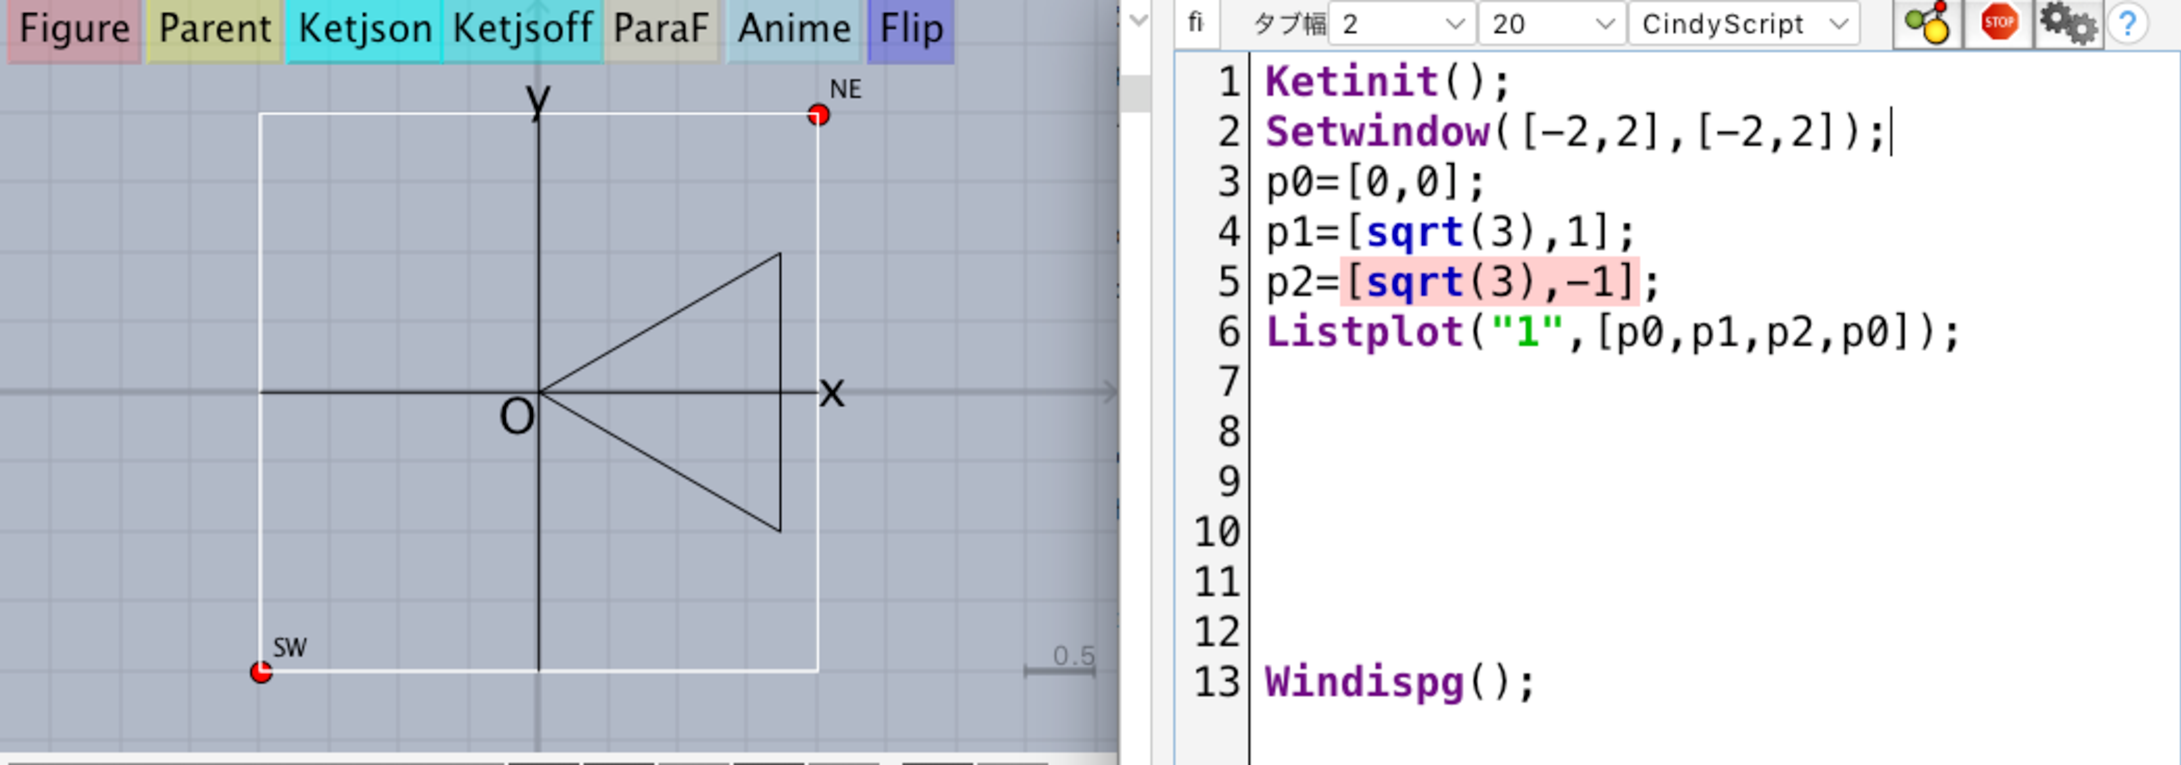
\includegraphics[bb=0.00 0.00 1047.00 367.00,width=120mm]{fig/sample1.pdf}}
\end{layer}

\vspace*{40mm}

%%%%%%%%%%%%

%%%%%%%%%%%%%%%%%%%%


\sameslide

\vspace*{18mm}

\slidepage

\begin{layer}{120}{0}
\putnotes{63}{5}{\scalebox{1}{%%% /Users/takatoosetsuo/specialclass.git/shibaura23/0607/presen/fig/sample1.tex 
%%% Generator=sample1.cdy 
{\unitlength=1cm%
\begin{picture}%
(4,4)(-2,-2)%
\linethickness{0.008in}%%
\polyline(0,0)(1.732,1)(1.732,-1)(0,0)%
%
\polyline(-2,0)(2,0)%
%
\polyline(0,-2)(0,2)%
%
\settowidth{\Width}{$x$}\setlength{\Width}{0\Width}%
\settoheight{\Height}{$x$}\settodepth{\Depth}{$x$}\setlength{\Height}{-0.5\Height}\setlength{\Depth}{0.5\Depth}\addtolength{\Height}{\Depth}%
\put(  2.050,  0.000){\hspace*{\Width}\raisebox{\Height}{$x$}}%
%
\settowidth{\Width}{$y$}\setlength{\Width}{-0.5\Width}%
\settoheight{\Height}{$y$}\settodepth{\Depth}{$y$}\setlength{\Height}{\Depth}%
\put(  0.000,  2.050){\hspace*{\Width}\raisebox{\Height}{$y$}}%
%
\settowidth{\Width}{O}\setlength{\Width}{-1\Width}%
\settoheight{\Height}{O}\settodepth{\Depth}{O}\setlength{\Height}{-\Height}%
\put( -0.050, -0.050){\hspace*{\Width}\raisebox{\Height}{O}}%
%
\end{picture}}%}}
\end{layer}

\vspace*{40mm}


\sameslide

\vspace*{18mm}

\slidepage

\begin{layer}{120}{0}
\putnotes{63}{5}{\scalebox{1}{%%% /Users/takatoosetsuo/specialclass.git/shibaura23/0607/presen/fig/sample1.tex 
%%% Generator=sample1.cdy 
{\unitlength=1cm%
\begin{picture}%
(4,4)(-2,-2)%
\linethickness{0.008in}%%
\polyline(0,0)(1.732,1)(1.732,-1)(0,0)%
%
\polyline(-2,0)(2,0)%
%
\polyline(0,-2)(0,2)%
%
\settowidth{\Width}{$x$}\setlength{\Width}{0\Width}%
\settoheight{\Height}{$x$}\settodepth{\Depth}{$x$}\setlength{\Height}{-0.5\Height}\setlength{\Depth}{0.5\Depth}\addtolength{\Height}{\Depth}%
\put(  2.050,  0.000){\hspace*{\Width}\raisebox{\Height}{$x$}}%
%
\settowidth{\Width}{$y$}\setlength{\Width}{-0.5\Width}%
\settoheight{\Height}{$y$}\settodepth{\Depth}{$y$}\setlength{\Height}{\Depth}%
\put(  0.000,  2.050){\hspace*{\Width}\raisebox{\Height}{$y$}}%
%
\settowidth{\Width}{O}\setlength{\Width}{-1\Width}%
\settoheight{\Height}{O}\settodepth{\Depth}{O}\setlength{\Height}{-\Height}%
\put( -0.050, -0.050){\hspace*{\Width}\raisebox{\Height}{O}}%
%
\end{picture}}%}}
\end{layer}

\vspace*{40mm}

\begin{itemize}
\item
\TeX のディストリビューション\\
\hspace*{2zw}TeXLive, KeTTeX(TeXLiveのサブセット版)
\end{itemize}

\sameslide

\vspace*{18mm}

\slidepage

\begin{layer}{120}{0}
\putnotes{63}{5}{\scalebox{1}{%%% /Users/takatoosetsuo/specialclass.git/shibaura23/0607/presen/fig/sample1.tex 
%%% Generator=sample1.cdy 
{\unitlength=1cm%
\begin{picture}%
(4,4)(-2,-2)%
\linethickness{0.008in}%%
\polyline(0,0)(1.732,1)(1.732,-1)(0,0)%
%
\polyline(-2,0)(2,0)%
%
\polyline(0,-2)(0,2)%
%
\settowidth{\Width}{$x$}\setlength{\Width}{0\Width}%
\settoheight{\Height}{$x$}\settodepth{\Depth}{$x$}\setlength{\Height}{-0.5\Height}\setlength{\Depth}{0.5\Depth}\addtolength{\Height}{\Depth}%
\put(  2.050,  0.000){\hspace*{\Width}\raisebox{\Height}{$x$}}%
%
\settowidth{\Width}{$y$}\setlength{\Width}{-0.5\Width}%
\settoheight{\Height}{$y$}\settodepth{\Depth}{$y$}\setlength{\Height}{\Depth}%
\put(  0.000,  2.050){\hspace*{\Width}\raisebox{\Height}{$y$}}%
%
\settowidth{\Width}{O}\setlength{\Width}{-1\Width}%
\settoheight{\Height}{O}\settodepth{\Depth}{O}\setlength{\Height}{-\Height}%
\put( -0.050, -0.050){\hspace*{\Width}\raisebox{\Height}{O}}%
%
\end{picture}}%}}
\end{layer}

\vspace*{40mm}

\begin{itemize}
\item
\TeX のディストリビューション\\
\hspace*{2zw}TeXLive, KeTTeX(TeXLiveのサブセット版)
\item
picture環境\\
\hspace*{2zw}Tpic,Pict2e,Tikz
\end{itemize}

\newslide{\ketcindy のインストール}

\vspace*{18mm}

\slidepage
\begin{itemize}
\item
\TeX, Cinderella, R, KeTCindyパッケージ\vspace{-2mm}
\end{itemize}
%%%%%%%%%%%%

%%%%%%%%%%%%%%%%%%%%


\sameslide

\vspace*{18mm}

\slidepage
\begin{itemize}
\item
\TeX, Cinderella, R, KeTCindyパッケージ\vspace{-2mm}
\item
Windowsの場合のみSumatra(PDFビューア)も\vspace{-2mm}
\end{itemize}

\sameslide

\vspace*{18mm}

\slidepage
\begin{itemize}
\item
\TeX, Cinderella, R, KeTCindyパッケージ\vspace{-2mm}
\item
Windowsの場合のみSumatra(PDFビューア)も\vspace{-2mm}
\item
実は,Maxima, gcc の呼び出しもできる\vspace{-2mm}
\end{itemize}

\sameslide

\vspace*{18mm}

\slidepage
\begin{itemize}
\item
\TeX, Cinderella, R, KeTCindyパッケージ\vspace{-2mm}
\item
Windowsの場合のみSumatra(PDFビューア)も\vspace{-2mm}
\item
実は,Maxima, gcc の呼び出しもできる\vspace{-2mm}
\item
\href{https://s-takato.github.io/ketcindyorg/indexj.html}{KeTCindy Home}を参照\vspace{-2mm}
\end{itemize}

\sameslide

\vspace*{18mm}

\slidepage
\begin{itemize}
\item
\TeX, Cinderella, R, KeTCindyパッケージ\vspace{-2mm}
\item
Windowsの場合のみSumatra(PDFビューア)も\vspace{-2mm}
\item
実は,Maxima, gcc の呼び出しもできる\vspace{-2mm}
\item
\href{https://s-takato.github.io/ketcindyorg/indexj.html}{KeTCindy Home}を参照\vspace{-2mm}
\item
[課題]\monban 使用しているシステムを教えて下さい\seteda{80}\\
\eda{WindowsかMacか}\\
\eda{OSの名前}
\end{itemize}

\newslide{KeTTeX のインストール}

\vspace*{18mm}

\slidepage

\begin{layer}{120}{0}
\putnotese{85}{30}{%%% Title presen0607
\documentclass[landscape,10pt]{ujarticle}
\special{papersize=\the\paperwidth,\the\paperheight}
\usepackage{ketpic,ketlayer}
\usepackage{ketslide}
\usepackage{amsmath,amssymb}
\usepackage{bm,enumerate}
\usepackage[dvipdfmx]{graphicx}
\usepackage{color}
\definecolor{slidecolora}{cmyk}{0.98,0.13,0,0.43}
\definecolor{slidecolorb}{cmyk}{0.2,0,0,0}
\definecolor{slidecolorc}{cmyk}{0.2,0,0,0}
\definecolor{slidecolord}{cmyk}{0.2,0,0,0}
\definecolor{slidecolore}{cmyk}{0,0,0,0.5}
\definecolor{slidecolorf}{cmyk}{0,0,0,0.5}
\definecolor{slidecolori}{cmyk}{0.98,0.13,0,0.43}
\def\setthin#1{\def\thin{#1}}
\setthin{0}
\newcommand{\slidepage}[1][s]{%
\setcounter{ketpicctra}{18}%
\if#1m \setcounter{ketpicctra}{1}\fi
\hypersetup{linkcolor=black}%

\begin{layer}{118}{0}
\putnotee{122}{-\theketpicctra.05}{\small\thepage/\pageref{pageend}}
\end{layer}\hypersetup{linkcolor=blue}

}
\usepackage{emath}
\usepackage{emathEy}
\usepackage{emathMw}
\usepackage{pict2e}
\usepackage{ketlayermorewith2e}
\usepackage[dvipdfmx,colorlinks=true,linkcolor=blue,filecolor=blue]{hyperref}
\newcommand{\hiduke}{0607}
\newcommand{\hako}[2][1]{\fbox{\raisebox{#1mm}{\mbox{}}\raisebox{-#1mm}{\mbox{}}\,\phantom{#2}\,}}
\newcommand{\hakoa}[2][1]{\fbox{\raisebox{#1mm}{\mbox{}}\raisebox{-#1mm}{\mbox{}}\,#2\,}}
\newcommand{\hakom}[2][1]{\hako[#1]{$#2$}}
\newcommand{\hakoma}[2][1]{\hakoa[#1]{$#2$}}
\def\rad{\;\mathrm{rad}}
\def\deg#1{#1^{\circ}}
\newcommand{\sbunsuu}[2]{\scalebox{0.6}{$\bunsuu{#1}{#2}$}}
\def\pow{$\hspace{-1.5mm}^\hspace{-1mm}$}
\def\dlim{\displaystyle\lim}
\newcommand{\brd}[2][1]{\scalebox{#1}{\color{red}\fbox{\color{black}$#2$}}}
\newcommand\down[1][0.5zw]{\vspace{#1}\\}
\newcommand{\sfrac}[3][0.65]{\scalebox{#1}{$\frac{#2}{#3}$}}
\newcommand{\phn}[1]{\phantom{#1}}
\newcommand{\scb}[2][0.6]{\scalebox{#1}{#2}}
\newcommand{\dsum}{\displaystyle\sum}

\setmargin{25}{145}{15}{100}

\ketslideinit

\pagestyle{empty}

\begin{document}

\begin{layer}{120}{0}
\putnotese{0}{0}{{\Large\bf
\color[cmyk]{1,1,0,0}

\begin{layer}{120}{0}
{\Huge \putnotes{60}{20}{インストール状況}}
\putnotes{60}{50}{高遠節夫}
\end{layer}

}
}
\end{layer}

\def\mainslidetitley{22}
\def\ketcletter{slidecolora}
\def\ketcbox{slidecolorb}
\def\ketdbox{slidecolorc}
\def\ketcframe{slidecolord}
\def\ketcshadow{slidecolore}
\def\ketdshadow{slidecolorf}
\def\slidetitlex{6}
\def\slidetitlesize{1.3}
\def\mketcletter{slidecolori}
\def\mketcbox{yellow}
\def\mketdbox{yellow}
\def\mketcframe{yellow}
\def\mslidetitlex{62}
\def\mslidetitlesize{2}

\color{black}
\Large\bf\boldmath
\addtocounter{page}{-1}

\def\MARU{}
\renewcommand{\MARU}[1]{{\ooalign{\hfil$#1$\/\hfil\crcr\raise.167ex\hbox{\mathhexbox20D}}}}
\renewcommand{\slidepage}[1][s]{%
\setcounter{ketpicctra}{18}%
\if#1m \setcounter{ketpicctra}{1}\fi
\hypersetup{linkcolor=black}%
\begin{layer}{118}{0}
\putnotee{115}{-\theketpicctra.05}{\small\hiduke-\thepage/\pageref{pageend}}
\end{layer}\hypersetup{linkcolor=blue}
}
\newcounter{ban}
\setcounter{ban}{1}
\newcommand{\monban}[1][\hiduke]{%
#1-\theban\ %
\addtocounter{ban}{1}%
}
\newcommand{\monbannoadd}[1][\hiduke]{%
#1-\theban\ %
}
\newcommand{\addban}{%
\addtocounter{ban}{1}%%210614
}
\newcounter{edawidth}
\newcounter{edactr}
\newcommand{\seteda}[1]{
\setcounter{edawidth}{#1}
\setcounter{edactr}{1}
}
\newcommand{\eda}[2][\theedawidth ]{%
\noindent\Ltab{#1 mm}{[\theedactr]\ #2}%
\addtocounter{edactr}{1}%
}
%%%%%%%%%%%%

%%%%%%%%%%%%%%%%%%%%

\mainslide{KeTCindy}


\slidepage[m]
%%%%%%%%%%%%
%%%%%%%%%%%%

%%%%%%%%%%%%%%%%%%%%

\newslide{\ketcindy とは}

\vspace*{18mm}

\slidepage
\begin{itemize}
\item
Cinderellaと連携して\TeX 用の図を作成
\item
\TeX のディストリビューション\\
\hspace*{2zw}TeXLive, KeTTeX(TeXLiveのサブセット版)
\item
picture環境\\
\hspace*{2zw}Tpic,Pict2e,Tikz
\item
Rとpdfビューアも用いる
\end{itemize}
%%%%%%%%%%%%

%%%%%%%%%%%%%%%%%%%%


\newslide{\ketcindy のインストール}

\vspace*{18mm}

\slidepage

\begin{layer}{120}{0}
\end{layer}

\begin{itemize}
\item
\TeX, Cinderella, R, KeTCindyパッケージ\vspace{-2mm}
\item
Windowsの場合のみSumatra(PDFビューア)も\vspace{-2mm}
\item
実は,Maxima, gcc の呼び出しもできる\vspace{-2mm}
\item
\href{https://s-takato.github.io/ketcindyorg/indexj.html}{KeTCindy Home}を参照\vspace{-2mm}
\end{itemize}

\sameslide

\vspace*{18mm}

\slidepage

\begin{layer}{120}{0}
\putnotese{85}{47}{%%% Title presen0607
\documentclass[landscape,10pt]{ujarticle}
\special{papersize=\the\paperwidth,\the\paperheight}
\usepackage{ketpic,ketlayer}
\usepackage{ketslide}
\usepackage{amsmath,amssymb}
\usepackage{bm,enumerate}
\usepackage[dvipdfmx]{graphicx}
\usepackage{color}
\definecolor{slidecolora}{cmyk}{0.98,0.13,0,0.43}
\definecolor{slidecolorb}{cmyk}{0.2,0,0,0}
\definecolor{slidecolorc}{cmyk}{0.2,0,0,0}
\definecolor{slidecolord}{cmyk}{0.2,0,0,0}
\definecolor{slidecolore}{cmyk}{0,0,0,0.5}
\definecolor{slidecolorf}{cmyk}{0,0,0,0.5}
\definecolor{slidecolori}{cmyk}{0.98,0.13,0,0.43}
\def\setthin#1{\def\thin{#1}}
\setthin{0}
\newcommand{\slidepage}[1][s]{%
\setcounter{ketpicctra}{18}%
\if#1m \setcounter{ketpicctra}{1}\fi
\hypersetup{linkcolor=black}%

\begin{layer}{118}{0}
\putnotee{122}{-\theketpicctra.05}{\small\thepage/\pageref{pageend}}
\end{layer}\hypersetup{linkcolor=blue}

}
\usepackage{emath}
\usepackage{emathEy}
\usepackage{emathMw}
\usepackage{pict2e}
\usepackage{ketlayermorewith2e}
\usepackage[dvipdfmx,colorlinks=true,linkcolor=blue,filecolor=blue]{hyperref}
\newcommand{\hiduke}{0607}
\newcommand{\hako}[2][1]{\fbox{\raisebox{#1mm}{\mbox{}}\raisebox{-#1mm}{\mbox{}}\,\phantom{#2}\,}}
\newcommand{\hakoa}[2][1]{\fbox{\raisebox{#1mm}{\mbox{}}\raisebox{-#1mm}{\mbox{}}\,#2\,}}
\newcommand{\hakom}[2][1]{\hako[#1]{$#2$}}
\newcommand{\hakoma}[2][1]{\hakoa[#1]{$#2$}}
\def\rad{\;\mathrm{rad}}
\def\deg#1{#1^{\circ}}
\newcommand{\sbunsuu}[2]{\scalebox{0.6}{$\bunsuu{#1}{#2}$}}
\def\pow{$\hspace{-1.5mm}^\hspace{-1mm}$}
\def\dlim{\displaystyle\lim}
\newcommand{\brd}[2][1]{\scalebox{#1}{\color{red}\fbox{\color{black}$#2$}}}
\newcommand\down[1][0.5zw]{\vspace{#1}\\}
\newcommand{\sfrac}[3][0.65]{\scalebox{#1}{$\frac{#2}{#3}$}}
\newcommand{\phn}[1]{\phantom{#1}}
\newcommand{\scb}[2][0.6]{\scalebox{#1}{#2}}
\newcommand{\dsum}{\displaystyle\sum}

\setmargin{25}{145}{15}{100}

\ketslideinit

\pagestyle{empty}

\begin{document}

\begin{layer}{120}{0}
\putnotese{0}{0}{{\Large\bf
\color[cmyk]{1,1,0,0}

\begin{layer}{120}{0}
{\Huge \putnotes{60}{20}{インストール状況}}
\putnotes{60}{50}{高遠節夫}
\end{layer}

}
}
\end{layer}

\def\mainslidetitley{22}
\def\ketcletter{slidecolora}
\def\ketcbox{slidecolorb}
\def\ketdbox{slidecolorc}
\def\ketcframe{slidecolord}
\def\ketcshadow{slidecolore}
\def\ketdshadow{slidecolorf}
\def\slidetitlex{6}
\def\slidetitlesize{1.3}
\def\mketcletter{slidecolori}
\def\mketcbox{yellow}
\def\mketdbox{yellow}
\def\mketcframe{yellow}
\def\mslidetitlex{62}
\def\mslidetitlesize{2}

\color{black}
\Large\bf\boldmath
\addtocounter{page}{-1}

\def\MARU{}
\renewcommand{\MARU}[1]{{\ooalign{\hfil$#1$\/\hfil\crcr\raise.167ex\hbox{\mathhexbox20D}}}}
\renewcommand{\slidepage}[1][s]{%
\setcounter{ketpicctra}{18}%
\if#1m \setcounter{ketpicctra}{1}\fi
\hypersetup{linkcolor=black}%
\begin{layer}{118}{0}
\putnotee{115}{-\theketpicctra.05}{\small\hiduke-\thepage/\pageref{pageend}}
\end{layer}\hypersetup{linkcolor=blue}
}
\newcounter{ban}
\setcounter{ban}{1}
\newcommand{\monban}[1][\hiduke]{%
#1-\theban\ %
\addtocounter{ban}{1}%
}
\newcommand{\monbannoadd}[1][\hiduke]{%
#1-\theban\ %
}
\newcommand{\addban}{%
\addtocounter{ban}{1}%%210614
}
\newcounter{edawidth}
\newcounter{edactr}
\newcommand{\seteda}[1]{
\setcounter{edawidth}{#1}
\setcounter{edactr}{1}
}
\newcommand{\eda}[2][\theedawidth ]{%
\noindent\Ltab{#1 mm}{[\theedactr]\ #2}%
\addtocounter{edactr}{1}%
}
%%%%%%%%%%%%

%%%%%%%%%%%%%%%%%%%%

\mainslide{KeTCindy}


\slidepage[m]
%%%%%%%%%%%%
%%%%%%%%%%%%

%%%%%%%%%%%%%%%%%%%%

\newslide{\ketcindy とは}

\vspace*{18mm}

\slidepage
\begin{itemize}
\item
Cinderellaと連携して\TeX 用の図を作成
\item
\TeX のディストリビューション\\
\hspace*{2zw}TeXLive, KeTTeX(TeXLiveのサブセット版)
\item
picture環境\\
\hspace*{2zw}Tpic,Pict2e,Tikz
\item
Rとpdfビューアも用いる
\end{itemize}
%%%%%%%%%%%%

%%%%%%%%%%%%%%%%%%%%


\newslide{\ketcindy のインストール}

\vspace*{18mm}

\slidepage

\begin{layer}{120}{0}
\end{layer}

\begin{itemize}
\item
\TeX, Cinderella, R, KeTCindyパッケージ\vspace{-2mm}
\item
Windowsの場合のみSumatra(PDFビューア)も\vspace{-2mm}
\item
実は,Maxima, gcc の呼び出しもできる\vspace{-2mm}
\item
\href{https://s-takato.github.io/ketcindyorg/indexj.html}{KeTCindy Home}を参照\vspace{-2mm}
\end{itemize}

\sameslide

\vspace*{18mm}

\slidepage

\begin{layer}{120}{0}
\putnotese{85}{47}{%%% Title presen0607
\documentclass[landscape,10pt]{ujarticle}
\special{papersize=\the\paperwidth,\the\paperheight}
\usepackage{ketpic,ketlayer}
\usepackage{ketslide}
\usepackage{amsmath,amssymb}
\usepackage{bm,enumerate}
\usepackage[dvipdfmx]{graphicx}
\usepackage{color}
\definecolor{slidecolora}{cmyk}{0.98,0.13,0,0.43}
\definecolor{slidecolorb}{cmyk}{0.2,0,0,0}
\definecolor{slidecolorc}{cmyk}{0.2,0,0,0}
\definecolor{slidecolord}{cmyk}{0.2,0,0,0}
\definecolor{slidecolore}{cmyk}{0,0,0,0.5}
\definecolor{slidecolorf}{cmyk}{0,0,0,0.5}
\definecolor{slidecolori}{cmyk}{0.98,0.13,0,0.43}
\def\setthin#1{\def\thin{#1}}
\setthin{0}
\newcommand{\slidepage}[1][s]{%
\setcounter{ketpicctra}{18}%
\if#1m \setcounter{ketpicctra}{1}\fi
\hypersetup{linkcolor=black}%

\begin{layer}{118}{0}
\putnotee{122}{-\theketpicctra.05}{\small\thepage/\pageref{pageend}}
\end{layer}\hypersetup{linkcolor=blue}

}
\usepackage{emath}
\usepackage{emathEy}
\usepackage{emathMw}
\usepackage{pict2e}
\usepackage{ketlayermorewith2e}
\usepackage[dvipdfmx,colorlinks=true,linkcolor=blue,filecolor=blue]{hyperref}
\newcommand{\hiduke}{0607}
\newcommand{\hako}[2][1]{\fbox{\raisebox{#1mm}{\mbox{}}\raisebox{-#1mm}{\mbox{}}\,\phantom{#2}\,}}
\newcommand{\hakoa}[2][1]{\fbox{\raisebox{#1mm}{\mbox{}}\raisebox{-#1mm}{\mbox{}}\,#2\,}}
\newcommand{\hakom}[2][1]{\hako[#1]{$#2$}}
\newcommand{\hakoma}[2][1]{\hakoa[#1]{$#2$}}
\def\rad{\;\mathrm{rad}}
\def\deg#1{#1^{\circ}}
\newcommand{\sbunsuu}[2]{\scalebox{0.6}{$\bunsuu{#1}{#2}$}}
\def\pow{$\hspace{-1.5mm}^\hspace{-1mm}$}
\def\dlim{\displaystyle\lim}
\newcommand{\brd}[2][1]{\scalebox{#1}{\color{red}\fbox{\color{black}$#2$}}}
\newcommand\down[1][0.5zw]{\vspace{#1}\\}
\newcommand{\sfrac}[3][0.65]{\scalebox{#1}{$\frac{#2}{#3}$}}
\newcommand{\phn}[1]{\phantom{#1}}
\newcommand{\scb}[2][0.6]{\scalebox{#1}{#2}}
\newcommand{\dsum}{\displaystyle\sum}

\setmargin{25}{145}{15}{100}

\ketslideinit

\pagestyle{empty}

\begin{document}

\begin{layer}{120}{0}
\putnotese{0}{0}{\input{fig/slide0.tex}}
\end{layer}

\def\mainslidetitley{22}
\def\ketcletter{slidecolora}
\def\ketcbox{slidecolorb}
\def\ketdbox{slidecolorc}
\def\ketcframe{slidecolord}
\def\ketcshadow{slidecolore}
\def\ketdshadow{slidecolorf}
\def\slidetitlex{6}
\def\slidetitlesize{1.3}
\def\mketcletter{slidecolori}
\def\mketcbox{yellow}
\def\mketdbox{yellow}
\def\mketcframe{yellow}
\def\mslidetitlex{62}
\def\mslidetitlesize{2}

\color{black}
\Large\bf\boldmath
\addtocounter{page}{-1}

\def\MARU{}
\renewcommand{\MARU}[1]{{\ooalign{\hfil$#1$\/\hfil\crcr\raise.167ex\hbox{\mathhexbox20D}}}}
\renewcommand{\slidepage}[1][s]{%
\setcounter{ketpicctra}{18}%
\if#1m \setcounter{ketpicctra}{1}\fi
\hypersetup{linkcolor=black}%
\begin{layer}{118}{0}
\putnotee{115}{-\theketpicctra.05}{\small\hiduke-\thepage/\pageref{pageend}}
\end{layer}\hypersetup{linkcolor=blue}
}
\newcounter{ban}
\setcounter{ban}{1}
\newcommand{\monban}[1][\hiduke]{%
#1-\theban\ %
\addtocounter{ban}{1}%
}
\newcommand{\monbannoadd}[1][\hiduke]{%
#1-\theban\ %
}
\newcommand{\addban}{%
\addtocounter{ban}{1}%%210614
}
\newcounter{edawidth}
\newcounter{edactr}
\newcommand{\seteda}[1]{
\setcounter{edawidth}{#1}
\setcounter{edactr}{1}
}
\newcommand{\eda}[2][\theedawidth ]{%
\noindent\Ltab{#1 mm}{[\theedactr]\ #2}%
\addtocounter{edactr}{1}%
}
%%%%%%%%%%%%

%%%%%%%%%%%%%%%%%%%%

\mainslide{KeTCindy}


\slidepage[m]
%%%%%%%%%%%%
%%%%%%%%%%%%

%%%%%%%%%%%%%%%%%%%%

\newslide{\ketcindy とは}

\vspace*{18mm}

\slidepage
\begin{itemize}
\item
Cinderellaと連携して\TeX 用の図を作成
\item
\TeX のディストリビューション\\
\hspace*{2zw}TeXLive, KeTTeX(TeXLiveのサブセット版)
\item
picture環境\\
\hspace*{2zw}Tpic,Pict2e,Tikz
\item
Rとpdfビューアも用いる
\end{itemize}
%%%%%%%%%%%%

%%%%%%%%%%%%%%%%%%%%


\newslide{\ketcindy のインストール}

\vspace*{18mm}

\slidepage

\begin{layer}{120}{0}
\end{layer}

\begin{itemize}
\item
\TeX, Cinderella, R, KeTCindyパッケージ\vspace{-2mm}
\item
Windowsの場合のみSumatra(PDFビューア)も\vspace{-2mm}
\item
実は,Maxima, gcc の呼び出しもできる\vspace{-2mm}
\item
\href{https://s-takato.github.io/ketcindyorg/indexj.html}{KeTCindy Home}を参照\vspace{-2mm}
\end{itemize}

\sameslide

\vspace*{18mm}

\slidepage

\begin{layer}{120}{0}
\putnotese{85}{47}{\input{fig/presen0607.tex}}
\end{layer}

\begin{itemize}
\item
\TeX, Cinderella, R, KeTCindyパッケージ\vspace{-2mm}
\item
Windowsの場合のみSumatra(PDFビューア)も\vspace{-2mm}
\item
実は,Maxima, gcc の呼び出しもできる\vspace{-2mm}
\item
\href{https://s-takato.github.io/ketcindyorg/indexj.html}{KeTCindy Home}を参照\vspace{-2mm}
\item
[課題]\monban インストールの状況(番号で)\\
コメントや質問(もしあったら)\seteda{35}\\
\eda[23]{TeX}\eda[37]{Cinderella}\eda{R}\\
\eda[40]{Sumatra}\eda{KeTCindy}
\end{itemize}
\label{pageend}\mbox{}

\end{document}
}
\end{layer}

\begin{itemize}
\item
\TeX, Cinderella, R, KeTCindyパッケージ\vspace{-2mm}
\item
Windowsの場合のみSumatra(PDFビューア)も\vspace{-2mm}
\item
実は,Maxima, gcc の呼び出しもできる\vspace{-2mm}
\item
\href{https://s-takato.github.io/ketcindyorg/indexj.html}{KeTCindy Home}を参照\vspace{-2mm}
\item
[課題]\monban インストールの状況(番号で)\\
コメントや質問(もしあったら)\seteda{35}\\
\eda[23]{TeX}\eda[37]{Cinderella}\eda{R}\\
\eda[40]{Sumatra}\eda{KeTCindy}
\end{itemize}
\label{pageend}\mbox{}

\end{document}
}
\end{layer}

\begin{itemize}
\item
\TeX, Cinderella, R, KeTCindyパッケージ\vspace{-2mm}
\item
Windowsの場合のみSumatra(PDFビューア)も\vspace{-2mm}
\item
実は,Maxima, gcc の呼び出しもできる\vspace{-2mm}
\item
\href{https://s-takato.github.io/ketcindyorg/indexj.html}{KeTCindy Home}を参照\vspace{-2mm}
\item
[課題]\monban インストールの状況(番号で)\\
コメントや質問(もしあったら)\seteda{35}\\
\eda[23]{TeX}\eda[37]{Cinderella}\eda{R}\\
\eda[40]{Sumatra}\eda{KeTCindy}
\end{itemize}
\label{pageend}\mbox{}

\end{document}
}
\end{layer}

\begin{itemize}
\item
[課題]\monban TeX インストールの状況\seteda{80}\\
\eda{状況の番号(表から)}\\
\eda{1,2の場合,詳細を説明してください}
\end{itemize}
%%%%%%%%%%%%

%%%%%%%%%%%%%%%%%%%%


\newslide{R(, Sumatra)のインストール}

\vspace*{18mm}

\slidepage

\begin{layer}{120}{0}
\putnotese{85}{30}{%%% Title presen0607
\documentclass[landscape,10pt]{ujarticle}
\special{papersize=\the\paperwidth,\the\paperheight}
\usepackage{ketpic,ketlayer}
\usepackage{ketslide}
\usepackage{amsmath,amssymb}
\usepackage{bm,enumerate}
\usepackage[dvipdfmx]{graphicx}
\usepackage{color}
\definecolor{slidecolora}{cmyk}{0.98,0.13,0,0.43}
\definecolor{slidecolorb}{cmyk}{0.2,0,0,0}
\definecolor{slidecolorc}{cmyk}{0.2,0,0,0}
\definecolor{slidecolord}{cmyk}{0.2,0,0,0}
\definecolor{slidecolore}{cmyk}{0,0,0,0.5}
\definecolor{slidecolorf}{cmyk}{0,0,0,0.5}
\definecolor{slidecolori}{cmyk}{0.98,0.13,0,0.43}
\def\setthin#1{\def\thin{#1}}
\setthin{0}
\newcommand{\slidepage}[1][s]{%
\setcounter{ketpicctra}{18}%
\if#1m \setcounter{ketpicctra}{1}\fi
\hypersetup{linkcolor=black}%

\begin{layer}{118}{0}
\putnotee{122}{-\theketpicctra.05}{\small\thepage/\pageref{pageend}}
\end{layer}\hypersetup{linkcolor=blue}

}
\usepackage{emath}
\usepackage{emathEy}
\usepackage{emathMw}
\usepackage{pict2e}
\usepackage{ketlayermorewith2e}
\usepackage[dvipdfmx,colorlinks=true,linkcolor=blue,filecolor=blue]{hyperref}
\newcommand{\hiduke}{0607}
\newcommand{\hako}[2][1]{\fbox{\raisebox{#1mm}{\mbox{}}\raisebox{-#1mm}{\mbox{}}\,\phantom{#2}\,}}
\newcommand{\hakoa}[2][1]{\fbox{\raisebox{#1mm}{\mbox{}}\raisebox{-#1mm}{\mbox{}}\,#2\,}}
\newcommand{\hakom}[2][1]{\hako[#1]{$#2$}}
\newcommand{\hakoma}[2][1]{\hakoa[#1]{$#2$}}
\def\rad{\;\mathrm{rad}}
\def\deg#1{#1^{\circ}}
\newcommand{\sbunsuu}[2]{\scalebox{0.6}{$\bunsuu{#1}{#2}$}}
\def\pow{$\hspace{-1.5mm}^\hspace{-1mm}$}
\def\dlim{\displaystyle\lim}
\newcommand{\brd}[2][1]{\scalebox{#1}{\color{red}\fbox{\color{black}$#2$}}}
\newcommand\down[1][0.5zw]{\vspace{#1}\\}
\newcommand{\sfrac}[3][0.65]{\scalebox{#1}{$\frac{#2}{#3}$}}
\newcommand{\phn}[1]{\phantom{#1}}
\newcommand{\scb}[2][0.6]{\scalebox{#1}{#2}}
\newcommand{\dsum}{\displaystyle\sum}

\setmargin{25}{145}{15}{100}

\ketslideinit

\pagestyle{empty}

\begin{document}

\begin{layer}{120}{0}
\putnotese{0}{0}{{\Large\bf
\color[cmyk]{1,1,0,0}

\begin{layer}{120}{0}
{\Huge \putnotes{60}{20}{インストール状況}}
\putnotes{60}{50}{高遠節夫}
\end{layer}

}
}
\end{layer}

\def\mainslidetitley{22}
\def\ketcletter{slidecolora}
\def\ketcbox{slidecolorb}
\def\ketdbox{slidecolorc}
\def\ketcframe{slidecolord}
\def\ketcshadow{slidecolore}
\def\ketdshadow{slidecolorf}
\def\slidetitlex{6}
\def\slidetitlesize{1.3}
\def\mketcletter{slidecolori}
\def\mketcbox{yellow}
\def\mketdbox{yellow}
\def\mketcframe{yellow}
\def\mslidetitlex{62}
\def\mslidetitlesize{2}

\color{black}
\Large\bf\boldmath
\addtocounter{page}{-1}

\def\MARU{}
\renewcommand{\MARU}[1]{{\ooalign{\hfil$#1$\/\hfil\crcr\raise.167ex\hbox{\mathhexbox20D}}}}
\renewcommand{\slidepage}[1][s]{%
\setcounter{ketpicctra}{18}%
\if#1m \setcounter{ketpicctra}{1}\fi
\hypersetup{linkcolor=black}%
\begin{layer}{118}{0}
\putnotee{115}{-\theketpicctra.05}{\small\hiduke-\thepage/\pageref{pageend}}
\end{layer}\hypersetup{linkcolor=blue}
}
\newcounter{ban}
\setcounter{ban}{1}
\newcommand{\monban}[1][\hiduke]{%
#1-\theban\ %
\addtocounter{ban}{1}%
}
\newcommand{\monbannoadd}[1][\hiduke]{%
#1-\theban\ %
}
\newcommand{\addban}{%
\addtocounter{ban}{1}%%210614
}
\newcounter{edawidth}
\newcounter{edactr}
\newcommand{\seteda}[1]{
\setcounter{edawidth}{#1}
\setcounter{edactr}{1}
}
\newcommand{\eda}[2][\theedawidth ]{%
\noindent\Ltab{#1 mm}{[\theedactr]\ #2}%
\addtocounter{edactr}{1}%
}
%%%%%%%%%%%%

%%%%%%%%%%%%%%%%%%%%

\mainslide{KeTCindy}


\slidepage[m]
%%%%%%%%%%%%
%%%%%%%%%%%%

%%%%%%%%%%%%%%%%%%%%

\newslide{\ketcindy とは}

\vspace*{18mm}

\slidepage
\begin{itemize}
\item
Cinderellaと連携して\TeX 用の図を作成
\item
\TeX のディストリビューション\\
\hspace*{2zw}TeXLive, KeTTeX(TeXLiveのサブセット版)
\item
picture環境\\
\hspace*{2zw}Tpic,Pict2e,Tikz
\item
Rとpdfビューアも用いる
\end{itemize}
%%%%%%%%%%%%

%%%%%%%%%%%%%%%%%%%%


\newslide{\ketcindy のインストール}

\vspace*{18mm}

\slidepage

\begin{layer}{120}{0}
\end{layer}

\begin{itemize}
\item
\TeX, Cinderella, R, KeTCindyパッケージ\vspace{-2mm}
\item
Windowsの場合のみSumatra(PDFビューア)も\vspace{-2mm}
\item
実は,Maxima, gcc の呼び出しもできる\vspace{-2mm}
\item
\href{https://s-takato.github.io/ketcindyorg/indexj.html}{KeTCindy Home}を参照\vspace{-2mm}
\end{itemize}

\sameslide

\vspace*{18mm}

\slidepage

\begin{layer}{120}{0}
\putnotese{85}{47}{%%% Title presen0607
\documentclass[landscape,10pt]{ujarticle}
\special{papersize=\the\paperwidth,\the\paperheight}
\usepackage{ketpic,ketlayer}
\usepackage{ketslide}
\usepackage{amsmath,amssymb}
\usepackage{bm,enumerate}
\usepackage[dvipdfmx]{graphicx}
\usepackage{color}
\definecolor{slidecolora}{cmyk}{0.98,0.13,0,0.43}
\definecolor{slidecolorb}{cmyk}{0.2,0,0,0}
\definecolor{slidecolorc}{cmyk}{0.2,0,0,0}
\definecolor{slidecolord}{cmyk}{0.2,0,0,0}
\definecolor{slidecolore}{cmyk}{0,0,0,0.5}
\definecolor{slidecolorf}{cmyk}{0,0,0,0.5}
\definecolor{slidecolori}{cmyk}{0.98,0.13,0,0.43}
\def\setthin#1{\def\thin{#1}}
\setthin{0}
\newcommand{\slidepage}[1][s]{%
\setcounter{ketpicctra}{18}%
\if#1m \setcounter{ketpicctra}{1}\fi
\hypersetup{linkcolor=black}%

\begin{layer}{118}{0}
\putnotee{122}{-\theketpicctra.05}{\small\thepage/\pageref{pageend}}
\end{layer}\hypersetup{linkcolor=blue}

}
\usepackage{emath}
\usepackage{emathEy}
\usepackage{emathMw}
\usepackage{pict2e}
\usepackage{ketlayermorewith2e}
\usepackage[dvipdfmx,colorlinks=true,linkcolor=blue,filecolor=blue]{hyperref}
\newcommand{\hiduke}{0607}
\newcommand{\hako}[2][1]{\fbox{\raisebox{#1mm}{\mbox{}}\raisebox{-#1mm}{\mbox{}}\,\phantom{#2}\,}}
\newcommand{\hakoa}[2][1]{\fbox{\raisebox{#1mm}{\mbox{}}\raisebox{-#1mm}{\mbox{}}\,#2\,}}
\newcommand{\hakom}[2][1]{\hako[#1]{$#2$}}
\newcommand{\hakoma}[2][1]{\hakoa[#1]{$#2$}}
\def\rad{\;\mathrm{rad}}
\def\deg#1{#1^{\circ}}
\newcommand{\sbunsuu}[2]{\scalebox{0.6}{$\bunsuu{#1}{#2}$}}
\def\pow{$\hspace{-1.5mm}^\hspace{-1mm}$}
\def\dlim{\displaystyle\lim}
\newcommand{\brd}[2][1]{\scalebox{#1}{\color{red}\fbox{\color{black}$#2$}}}
\newcommand\down[1][0.5zw]{\vspace{#1}\\}
\newcommand{\sfrac}[3][0.65]{\scalebox{#1}{$\frac{#2}{#3}$}}
\newcommand{\phn}[1]{\phantom{#1}}
\newcommand{\scb}[2][0.6]{\scalebox{#1}{#2}}
\newcommand{\dsum}{\displaystyle\sum}

\setmargin{25}{145}{15}{100}

\ketslideinit

\pagestyle{empty}

\begin{document}

\begin{layer}{120}{0}
\putnotese{0}{0}{{\Large\bf
\color[cmyk]{1,1,0,0}

\begin{layer}{120}{0}
{\Huge \putnotes{60}{20}{インストール状況}}
\putnotes{60}{50}{高遠節夫}
\end{layer}

}
}
\end{layer}

\def\mainslidetitley{22}
\def\ketcletter{slidecolora}
\def\ketcbox{slidecolorb}
\def\ketdbox{slidecolorc}
\def\ketcframe{slidecolord}
\def\ketcshadow{slidecolore}
\def\ketdshadow{slidecolorf}
\def\slidetitlex{6}
\def\slidetitlesize{1.3}
\def\mketcletter{slidecolori}
\def\mketcbox{yellow}
\def\mketdbox{yellow}
\def\mketcframe{yellow}
\def\mslidetitlex{62}
\def\mslidetitlesize{2}

\color{black}
\Large\bf\boldmath
\addtocounter{page}{-1}

\def\MARU{}
\renewcommand{\MARU}[1]{{\ooalign{\hfil$#1$\/\hfil\crcr\raise.167ex\hbox{\mathhexbox20D}}}}
\renewcommand{\slidepage}[1][s]{%
\setcounter{ketpicctra}{18}%
\if#1m \setcounter{ketpicctra}{1}\fi
\hypersetup{linkcolor=black}%
\begin{layer}{118}{0}
\putnotee{115}{-\theketpicctra.05}{\small\hiduke-\thepage/\pageref{pageend}}
\end{layer}\hypersetup{linkcolor=blue}
}
\newcounter{ban}
\setcounter{ban}{1}
\newcommand{\monban}[1][\hiduke]{%
#1-\theban\ %
\addtocounter{ban}{1}%
}
\newcommand{\monbannoadd}[1][\hiduke]{%
#1-\theban\ %
}
\newcommand{\addban}{%
\addtocounter{ban}{1}%%210614
}
\newcounter{edawidth}
\newcounter{edactr}
\newcommand{\seteda}[1]{
\setcounter{edawidth}{#1}
\setcounter{edactr}{1}
}
\newcommand{\eda}[2][\theedawidth ]{%
\noindent\Ltab{#1 mm}{[\theedactr]\ #2}%
\addtocounter{edactr}{1}%
}
%%%%%%%%%%%%

%%%%%%%%%%%%%%%%%%%%

\mainslide{KeTCindy}


\slidepage[m]
%%%%%%%%%%%%
%%%%%%%%%%%%

%%%%%%%%%%%%%%%%%%%%

\newslide{\ketcindy とは}

\vspace*{18mm}

\slidepage
\begin{itemize}
\item
Cinderellaと連携して\TeX 用の図を作成
\item
\TeX のディストリビューション\\
\hspace*{2zw}TeXLive, KeTTeX(TeXLiveのサブセット版)
\item
picture環境\\
\hspace*{2zw}Tpic,Pict2e,Tikz
\item
Rとpdfビューアも用いる
\end{itemize}
%%%%%%%%%%%%

%%%%%%%%%%%%%%%%%%%%


\newslide{\ketcindy のインストール}

\vspace*{18mm}

\slidepage

\begin{layer}{120}{0}
\end{layer}

\begin{itemize}
\item
\TeX, Cinderella, R, KeTCindyパッケージ\vspace{-2mm}
\item
Windowsの場合のみSumatra(PDFビューア)も\vspace{-2mm}
\item
実は,Maxima, gcc の呼び出しもできる\vspace{-2mm}
\item
\href{https://s-takato.github.io/ketcindyorg/indexj.html}{KeTCindy Home}を参照\vspace{-2mm}
\end{itemize}

\sameslide

\vspace*{18mm}

\slidepage

\begin{layer}{120}{0}
\putnotese{85}{47}{%%% Title presen0607
\documentclass[landscape,10pt]{ujarticle}
\special{papersize=\the\paperwidth,\the\paperheight}
\usepackage{ketpic,ketlayer}
\usepackage{ketslide}
\usepackage{amsmath,amssymb}
\usepackage{bm,enumerate}
\usepackage[dvipdfmx]{graphicx}
\usepackage{color}
\definecolor{slidecolora}{cmyk}{0.98,0.13,0,0.43}
\definecolor{slidecolorb}{cmyk}{0.2,0,0,0}
\definecolor{slidecolorc}{cmyk}{0.2,0,0,0}
\definecolor{slidecolord}{cmyk}{0.2,0,0,0}
\definecolor{slidecolore}{cmyk}{0,0,0,0.5}
\definecolor{slidecolorf}{cmyk}{0,0,0,0.5}
\definecolor{slidecolori}{cmyk}{0.98,0.13,0,0.43}
\def\setthin#1{\def\thin{#1}}
\setthin{0}
\newcommand{\slidepage}[1][s]{%
\setcounter{ketpicctra}{18}%
\if#1m \setcounter{ketpicctra}{1}\fi
\hypersetup{linkcolor=black}%

\begin{layer}{118}{0}
\putnotee{122}{-\theketpicctra.05}{\small\thepage/\pageref{pageend}}
\end{layer}\hypersetup{linkcolor=blue}

}
\usepackage{emath}
\usepackage{emathEy}
\usepackage{emathMw}
\usepackage{pict2e}
\usepackage{ketlayermorewith2e}
\usepackage[dvipdfmx,colorlinks=true,linkcolor=blue,filecolor=blue]{hyperref}
\newcommand{\hiduke}{0607}
\newcommand{\hako}[2][1]{\fbox{\raisebox{#1mm}{\mbox{}}\raisebox{-#1mm}{\mbox{}}\,\phantom{#2}\,}}
\newcommand{\hakoa}[2][1]{\fbox{\raisebox{#1mm}{\mbox{}}\raisebox{-#1mm}{\mbox{}}\,#2\,}}
\newcommand{\hakom}[2][1]{\hako[#1]{$#2$}}
\newcommand{\hakoma}[2][1]{\hakoa[#1]{$#2$}}
\def\rad{\;\mathrm{rad}}
\def\deg#1{#1^{\circ}}
\newcommand{\sbunsuu}[2]{\scalebox{0.6}{$\bunsuu{#1}{#2}$}}
\def\pow{$\hspace{-1.5mm}^\hspace{-1mm}$}
\def\dlim{\displaystyle\lim}
\newcommand{\brd}[2][1]{\scalebox{#1}{\color{red}\fbox{\color{black}$#2$}}}
\newcommand\down[1][0.5zw]{\vspace{#1}\\}
\newcommand{\sfrac}[3][0.65]{\scalebox{#1}{$\frac{#2}{#3}$}}
\newcommand{\phn}[1]{\phantom{#1}}
\newcommand{\scb}[2][0.6]{\scalebox{#1}{#2}}
\newcommand{\dsum}{\displaystyle\sum}

\setmargin{25}{145}{15}{100}

\ketslideinit

\pagestyle{empty}

\begin{document}

\begin{layer}{120}{0}
\putnotese{0}{0}{\input{fig/slide0.tex}}
\end{layer}

\def\mainslidetitley{22}
\def\ketcletter{slidecolora}
\def\ketcbox{slidecolorb}
\def\ketdbox{slidecolorc}
\def\ketcframe{slidecolord}
\def\ketcshadow{slidecolore}
\def\ketdshadow{slidecolorf}
\def\slidetitlex{6}
\def\slidetitlesize{1.3}
\def\mketcletter{slidecolori}
\def\mketcbox{yellow}
\def\mketdbox{yellow}
\def\mketcframe{yellow}
\def\mslidetitlex{62}
\def\mslidetitlesize{2}

\color{black}
\Large\bf\boldmath
\addtocounter{page}{-1}

\def\MARU{}
\renewcommand{\MARU}[1]{{\ooalign{\hfil$#1$\/\hfil\crcr\raise.167ex\hbox{\mathhexbox20D}}}}
\renewcommand{\slidepage}[1][s]{%
\setcounter{ketpicctra}{18}%
\if#1m \setcounter{ketpicctra}{1}\fi
\hypersetup{linkcolor=black}%
\begin{layer}{118}{0}
\putnotee{115}{-\theketpicctra.05}{\small\hiduke-\thepage/\pageref{pageend}}
\end{layer}\hypersetup{linkcolor=blue}
}
\newcounter{ban}
\setcounter{ban}{1}
\newcommand{\monban}[1][\hiduke]{%
#1-\theban\ %
\addtocounter{ban}{1}%
}
\newcommand{\monbannoadd}[1][\hiduke]{%
#1-\theban\ %
}
\newcommand{\addban}{%
\addtocounter{ban}{1}%%210614
}
\newcounter{edawidth}
\newcounter{edactr}
\newcommand{\seteda}[1]{
\setcounter{edawidth}{#1}
\setcounter{edactr}{1}
}
\newcommand{\eda}[2][\theedawidth ]{%
\noindent\Ltab{#1 mm}{[\theedactr]\ #2}%
\addtocounter{edactr}{1}%
}
%%%%%%%%%%%%

%%%%%%%%%%%%%%%%%%%%

\mainslide{KeTCindy}


\slidepage[m]
%%%%%%%%%%%%
%%%%%%%%%%%%

%%%%%%%%%%%%%%%%%%%%

\newslide{\ketcindy とは}

\vspace*{18mm}

\slidepage
\begin{itemize}
\item
Cinderellaと連携して\TeX 用の図を作成
\item
\TeX のディストリビューション\\
\hspace*{2zw}TeXLive, KeTTeX(TeXLiveのサブセット版)
\item
picture環境\\
\hspace*{2zw}Tpic,Pict2e,Tikz
\item
Rとpdfビューアも用いる
\end{itemize}
%%%%%%%%%%%%

%%%%%%%%%%%%%%%%%%%%


\newslide{\ketcindy のインストール}

\vspace*{18mm}

\slidepage

\begin{layer}{120}{0}
\end{layer}

\begin{itemize}
\item
\TeX, Cinderella, R, KeTCindyパッケージ\vspace{-2mm}
\item
Windowsの場合のみSumatra(PDFビューア)も\vspace{-2mm}
\item
実は,Maxima, gcc の呼び出しもできる\vspace{-2mm}
\item
\href{https://s-takato.github.io/ketcindyorg/indexj.html}{KeTCindy Home}を参照\vspace{-2mm}
\end{itemize}

\sameslide

\vspace*{18mm}

\slidepage

\begin{layer}{120}{0}
\putnotese{85}{47}{\input{fig/presen0607.tex}}
\end{layer}

\begin{itemize}
\item
\TeX, Cinderella, R, KeTCindyパッケージ\vspace{-2mm}
\item
Windowsの場合のみSumatra(PDFビューア)も\vspace{-2mm}
\item
実は,Maxima, gcc の呼び出しもできる\vspace{-2mm}
\item
\href{https://s-takato.github.io/ketcindyorg/indexj.html}{KeTCindy Home}を参照\vspace{-2mm}
\item
[課題]\monban インストールの状況(番号で)\\
コメントや質問(もしあったら)\seteda{35}\\
\eda[23]{TeX}\eda[37]{Cinderella}\eda{R}\\
\eda[40]{Sumatra}\eda{KeTCindy}
\end{itemize}
\label{pageend}\mbox{}

\end{document}
}
\end{layer}

\begin{itemize}
\item
\TeX, Cinderella, R, KeTCindyパッケージ\vspace{-2mm}
\item
Windowsの場合のみSumatra(PDFビューア)も\vspace{-2mm}
\item
実は,Maxima, gcc の呼び出しもできる\vspace{-2mm}
\item
\href{https://s-takato.github.io/ketcindyorg/indexj.html}{KeTCindy Home}を参照\vspace{-2mm}
\item
[課題]\monban インストールの状況(番号で)\\
コメントや質問(もしあったら)\seteda{35}\\
\eda[23]{TeX}\eda[37]{Cinderella}\eda{R}\\
\eda[40]{Sumatra}\eda{KeTCindy}
\end{itemize}
\label{pageend}\mbox{}

\end{document}
}
\end{layer}

\begin{itemize}
\item
\TeX, Cinderella, R, KeTCindyパッケージ\vspace{-2mm}
\item
Windowsの場合のみSumatra(PDFビューア)も\vspace{-2mm}
\item
実は,Maxima, gcc の呼び出しもできる\vspace{-2mm}
\item
\href{https://s-takato.github.io/ketcindyorg/indexj.html}{KeTCindy Home}を参照\vspace{-2mm}
\item
[課題]\monban インストールの状況(番号で)\\
コメントや質問(もしあったら)\seteda{35}\\
\eda[23]{TeX}\eda[37]{Cinderella}\eda{R}\\
\eda[40]{Sumatra}\eda{KeTCindy}
\end{itemize}
\label{pageend}\mbox{}

\end{document}
}
\end{layer}

\begin{itemize}
\item
[課題]\monban R(, Sumatra) インストールの状況\seteda{80}\\
\eda{状況の番号(表から)}\\
\eda{1,2の場合,詳細を説明してください}
\end{itemize}
%%%%%%%%%%%%

%%%%%%%%%%%%%%%%%%%%


\newslide{Cinderella のインストール}

\vspace*{18mm}

\slidepage

\begin{layer}{120}{0}
\putnotese{85}{30}{%%% Title presen0607
\documentclass[landscape,10pt]{ujarticle}
\special{papersize=\the\paperwidth,\the\paperheight}
\usepackage{ketpic,ketlayer}
\usepackage{ketslide}
\usepackage{amsmath,amssymb}
\usepackage{bm,enumerate}
\usepackage[dvipdfmx]{graphicx}
\usepackage{color}
\definecolor{slidecolora}{cmyk}{0.98,0.13,0,0.43}
\definecolor{slidecolorb}{cmyk}{0.2,0,0,0}
\definecolor{slidecolorc}{cmyk}{0.2,0,0,0}
\definecolor{slidecolord}{cmyk}{0.2,0,0,0}
\definecolor{slidecolore}{cmyk}{0,0,0,0.5}
\definecolor{slidecolorf}{cmyk}{0,0,0,0.5}
\definecolor{slidecolori}{cmyk}{0.98,0.13,0,0.43}
\def\setthin#1{\def\thin{#1}}
\setthin{0}
\newcommand{\slidepage}[1][s]{%
\setcounter{ketpicctra}{18}%
\if#1m \setcounter{ketpicctra}{1}\fi
\hypersetup{linkcolor=black}%

\begin{layer}{118}{0}
\putnotee{122}{-\theketpicctra.05}{\small\thepage/\pageref{pageend}}
\end{layer}\hypersetup{linkcolor=blue}

}
\usepackage{emath}
\usepackage{emathEy}
\usepackage{emathMw}
\usepackage{pict2e}
\usepackage{ketlayermorewith2e}
\usepackage[dvipdfmx,colorlinks=true,linkcolor=blue,filecolor=blue]{hyperref}
\newcommand{\hiduke}{0607}
\newcommand{\hako}[2][1]{\fbox{\raisebox{#1mm}{\mbox{}}\raisebox{-#1mm}{\mbox{}}\,\phantom{#2}\,}}
\newcommand{\hakoa}[2][1]{\fbox{\raisebox{#1mm}{\mbox{}}\raisebox{-#1mm}{\mbox{}}\,#2\,}}
\newcommand{\hakom}[2][1]{\hako[#1]{$#2$}}
\newcommand{\hakoma}[2][1]{\hakoa[#1]{$#2$}}
\def\rad{\;\mathrm{rad}}
\def\deg#1{#1^{\circ}}
\newcommand{\sbunsuu}[2]{\scalebox{0.6}{$\bunsuu{#1}{#2}$}}
\def\pow{$\hspace{-1.5mm}^\hspace{-1mm}$}
\def\dlim{\displaystyle\lim}
\newcommand{\brd}[2][1]{\scalebox{#1}{\color{red}\fbox{\color{black}$#2$}}}
\newcommand\down[1][0.5zw]{\vspace{#1}\\}
\newcommand{\sfrac}[3][0.65]{\scalebox{#1}{$\frac{#2}{#3}$}}
\newcommand{\phn}[1]{\phantom{#1}}
\newcommand{\scb}[2][0.6]{\scalebox{#1}{#2}}
\newcommand{\dsum}{\displaystyle\sum}

\setmargin{25}{145}{15}{100}

\ketslideinit

\pagestyle{empty}

\begin{document}

\begin{layer}{120}{0}
\putnotese{0}{0}{{\Large\bf
\color[cmyk]{1,1,0,0}

\begin{layer}{120}{0}
{\Huge \putnotes{60}{20}{インストール状況}}
\putnotes{60}{50}{高遠節夫}
\end{layer}

}
}
\end{layer}

\def\mainslidetitley{22}
\def\ketcletter{slidecolora}
\def\ketcbox{slidecolorb}
\def\ketdbox{slidecolorc}
\def\ketcframe{slidecolord}
\def\ketcshadow{slidecolore}
\def\ketdshadow{slidecolorf}
\def\slidetitlex{6}
\def\slidetitlesize{1.3}
\def\mketcletter{slidecolori}
\def\mketcbox{yellow}
\def\mketdbox{yellow}
\def\mketcframe{yellow}
\def\mslidetitlex{62}
\def\mslidetitlesize{2}

\color{black}
\Large\bf\boldmath
\addtocounter{page}{-1}

\def\MARU{}
\renewcommand{\MARU}[1]{{\ooalign{\hfil$#1$\/\hfil\crcr\raise.167ex\hbox{\mathhexbox20D}}}}
\renewcommand{\slidepage}[1][s]{%
\setcounter{ketpicctra}{18}%
\if#1m \setcounter{ketpicctra}{1}\fi
\hypersetup{linkcolor=black}%
\begin{layer}{118}{0}
\putnotee{115}{-\theketpicctra.05}{\small\hiduke-\thepage/\pageref{pageend}}
\end{layer}\hypersetup{linkcolor=blue}
}
\newcounter{ban}
\setcounter{ban}{1}
\newcommand{\monban}[1][\hiduke]{%
#1-\theban\ %
\addtocounter{ban}{1}%
}
\newcommand{\monbannoadd}[1][\hiduke]{%
#1-\theban\ %
}
\newcommand{\addban}{%
\addtocounter{ban}{1}%%210614
}
\newcounter{edawidth}
\newcounter{edactr}
\newcommand{\seteda}[1]{
\setcounter{edawidth}{#1}
\setcounter{edactr}{1}
}
\newcommand{\eda}[2][\theedawidth ]{%
\noindent\Ltab{#1 mm}{[\theedactr]\ #2}%
\addtocounter{edactr}{1}%
}
%%%%%%%%%%%%

%%%%%%%%%%%%%%%%%%%%

\mainslide{KeTCindy}


\slidepage[m]
%%%%%%%%%%%%
%%%%%%%%%%%%

%%%%%%%%%%%%%%%%%%%%

\newslide{\ketcindy とは}

\vspace*{18mm}

\slidepage
\begin{itemize}
\item
Cinderellaと連携して\TeX 用の図を作成
\item
\TeX のディストリビューション\\
\hspace*{2zw}TeXLive, KeTTeX(TeXLiveのサブセット版)
\item
picture環境\\
\hspace*{2zw}Tpic,Pict2e,Tikz
\item
Rとpdfビューアも用いる
\end{itemize}
%%%%%%%%%%%%

%%%%%%%%%%%%%%%%%%%%


\newslide{\ketcindy のインストール}

\vspace*{18mm}

\slidepage

\begin{layer}{120}{0}
\end{layer}

\begin{itemize}
\item
\TeX, Cinderella, R, KeTCindyパッケージ\vspace{-2mm}
\item
Windowsの場合のみSumatra(PDFビューア)も\vspace{-2mm}
\item
実は,Maxima, gcc の呼び出しもできる\vspace{-2mm}
\item
\href{https://s-takato.github.io/ketcindyorg/indexj.html}{KeTCindy Home}を参照\vspace{-2mm}
\end{itemize}

\sameslide

\vspace*{18mm}

\slidepage

\begin{layer}{120}{0}
\putnotese{85}{47}{%%% Title presen0607
\documentclass[landscape,10pt]{ujarticle}
\special{papersize=\the\paperwidth,\the\paperheight}
\usepackage{ketpic,ketlayer}
\usepackage{ketslide}
\usepackage{amsmath,amssymb}
\usepackage{bm,enumerate}
\usepackage[dvipdfmx]{graphicx}
\usepackage{color}
\definecolor{slidecolora}{cmyk}{0.98,0.13,0,0.43}
\definecolor{slidecolorb}{cmyk}{0.2,0,0,0}
\definecolor{slidecolorc}{cmyk}{0.2,0,0,0}
\definecolor{slidecolord}{cmyk}{0.2,0,0,0}
\definecolor{slidecolore}{cmyk}{0,0,0,0.5}
\definecolor{slidecolorf}{cmyk}{0,0,0,0.5}
\definecolor{slidecolori}{cmyk}{0.98,0.13,0,0.43}
\def\setthin#1{\def\thin{#1}}
\setthin{0}
\newcommand{\slidepage}[1][s]{%
\setcounter{ketpicctra}{18}%
\if#1m \setcounter{ketpicctra}{1}\fi
\hypersetup{linkcolor=black}%

\begin{layer}{118}{0}
\putnotee{122}{-\theketpicctra.05}{\small\thepage/\pageref{pageend}}
\end{layer}\hypersetup{linkcolor=blue}

}
\usepackage{emath}
\usepackage{emathEy}
\usepackage{emathMw}
\usepackage{pict2e}
\usepackage{ketlayermorewith2e}
\usepackage[dvipdfmx,colorlinks=true,linkcolor=blue,filecolor=blue]{hyperref}
\newcommand{\hiduke}{0607}
\newcommand{\hako}[2][1]{\fbox{\raisebox{#1mm}{\mbox{}}\raisebox{-#1mm}{\mbox{}}\,\phantom{#2}\,}}
\newcommand{\hakoa}[2][1]{\fbox{\raisebox{#1mm}{\mbox{}}\raisebox{-#1mm}{\mbox{}}\,#2\,}}
\newcommand{\hakom}[2][1]{\hako[#1]{$#2$}}
\newcommand{\hakoma}[2][1]{\hakoa[#1]{$#2$}}
\def\rad{\;\mathrm{rad}}
\def\deg#1{#1^{\circ}}
\newcommand{\sbunsuu}[2]{\scalebox{0.6}{$\bunsuu{#1}{#2}$}}
\def\pow{$\hspace{-1.5mm}^\hspace{-1mm}$}
\def\dlim{\displaystyle\lim}
\newcommand{\brd}[2][1]{\scalebox{#1}{\color{red}\fbox{\color{black}$#2$}}}
\newcommand\down[1][0.5zw]{\vspace{#1}\\}
\newcommand{\sfrac}[3][0.65]{\scalebox{#1}{$\frac{#2}{#3}$}}
\newcommand{\phn}[1]{\phantom{#1}}
\newcommand{\scb}[2][0.6]{\scalebox{#1}{#2}}
\newcommand{\dsum}{\displaystyle\sum}

\setmargin{25}{145}{15}{100}

\ketslideinit

\pagestyle{empty}

\begin{document}

\begin{layer}{120}{0}
\putnotese{0}{0}{{\Large\bf
\color[cmyk]{1,1,0,0}

\begin{layer}{120}{0}
{\Huge \putnotes{60}{20}{インストール状況}}
\putnotes{60}{50}{高遠節夫}
\end{layer}

}
}
\end{layer}

\def\mainslidetitley{22}
\def\ketcletter{slidecolora}
\def\ketcbox{slidecolorb}
\def\ketdbox{slidecolorc}
\def\ketcframe{slidecolord}
\def\ketcshadow{slidecolore}
\def\ketdshadow{slidecolorf}
\def\slidetitlex{6}
\def\slidetitlesize{1.3}
\def\mketcletter{slidecolori}
\def\mketcbox{yellow}
\def\mketdbox{yellow}
\def\mketcframe{yellow}
\def\mslidetitlex{62}
\def\mslidetitlesize{2}

\color{black}
\Large\bf\boldmath
\addtocounter{page}{-1}

\def\MARU{}
\renewcommand{\MARU}[1]{{\ooalign{\hfil$#1$\/\hfil\crcr\raise.167ex\hbox{\mathhexbox20D}}}}
\renewcommand{\slidepage}[1][s]{%
\setcounter{ketpicctra}{18}%
\if#1m \setcounter{ketpicctra}{1}\fi
\hypersetup{linkcolor=black}%
\begin{layer}{118}{0}
\putnotee{115}{-\theketpicctra.05}{\small\hiduke-\thepage/\pageref{pageend}}
\end{layer}\hypersetup{linkcolor=blue}
}
\newcounter{ban}
\setcounter{ban}{1}
\newcommand{\monban}[1][\hiduke]{%
#1-\theban\ %
\addtocounter{ban}{1}%
}
\newcommand{\monbannoadd}[1][\hiduke]{%
#1-\theban\ %
}
\newcommand{\addban}{%
\addtocounter{ban}{1}%%210614
}
\newcounter{edawidth}
\newcounter{edactr}
\newcommand{\seteda}[1]{
\setcounter{edawidth}{#1}
\setcounter{edactr}{1}
}
\newcommand{\eda}[2][\theedawidth ]{%
\noindent\Ltab{#1 mm}{[\theedactr]\ #2}%
\addtocounter{edactr}{1}%
}
%%%%%%%%%%%%

%%%%%%%%%%%%%%%%%%%%

\mainslide{KeTCindy}


\slidepage[m]
%%%%%%%%%%%%
%%%%%%%%%%%%

%%%%%%%%%%%%%%%%%%%%

\newslide{\ketcindy とは}

\vspace*{18mm}

\slidepage
\begin{itemize}
\item
Cinderellaと連携して\TeX 用の図を作成
\item
\TeX のディストリビューション\\
\hspace*{2zw}TeXLive, KeTTeX(TeXLiveのサブセット版)
\item
picture環境\\
\hspace*{2zw}Tpic,Pict2e,Tikz
\item
Rとpdfビューアも用いる
\end{itemize}
%%%%%%%%%%%%

%%%%%%%%%%%%%%%%%%%%


\newslide{\ketcindy のインストール}

\vspace*{18mm}

\slidepage

\begin{layer}{120}{0}
\end{layer}

\begin{itemize}
\item
\TeX, Cinderella, R, KeTCindyパッケージ\vspace{-2mm}
\item
Windowsの場合のみSumatra(PDFビューア)も\vspace{-2mm}
\item
実は,Maxima, gcc の呼び出しもできる\vspace{-2mm}
\item
\href{https://s-takato.github.io/ketcindyorg/indexj.html}{KeTCindy Home}を参照\vspace{-2mm}
\end{itemize}

\sameslide

\vspace*{18mm}

\slidepage

\begin{layer}{120}{0}
\putnotese{85}{47}{%%% Title presen0607
\documentclass[landscape,10pt]{ujarticle}
\special{papersize=\the\paperwidth,\the\paperheight}
\usepackage{ketpic,ketlayer}
\usepackage{ketslide}
\usepackage{amsmath,amssymb}
\usepackage{bm,enumerate}
\usepackage[dvipdfmx]{graphicx}
\usepackage{color}
\definecolor{slidecolora}{cmyk}{0.98,0.13,0,0.43}
\definecolor{slidecolorb}{cmyk}{0.2,0,0,0}
\definecolor{slidecolorc}{cmyk}{0.2,0,0,0}
\definecolor{slidecolord}{cmyk}{0.2,0,0,0}
\definecolor{slidecolore}{cmyk}{0,0,0,0.5}
\definecolor{slidecolorf}{cmyk}{0,0,0,0.5}
\definecolor{slidecolori}{cmyk}{0.98,0.13,0,0.43}
\def\setthin#1{\def\thin{#1}}
\setthin{0}
\newcommand{\slidepage}[1][s]{%
\setcounter{ketpicctra}{18}%
\if#1m \setcounter{ketpicctra}{1}\fi
\hypersetup{linkcolor=black}%

\begin{layer}{118}{0}
\putnotee{122}{-\theketpicctra.05}{\small\thepage/\pageref{pageend}}
\end{layer}\hypersetup{linkcolor=blue}

}
\usepackage{emath}
\usepackage{emathEy}
\usepackage{emathMw}
\usepackage{pict2e}
\usepackage{ketlayermorewith2e}
\usepackage[dvipdfmx,colorlinks=true,linkcolor=blue,filecolor=blue]{hyperref}
\newcommand{\hiduke}{0607}
\newcommand{\hako}[2][1]{\fbox{\raisebox{#1mm}{\mbox{}}\raisebox{-#1mm}{\mbox{}}\,\phantom{#2}\,}}
\newcommand{\hakoa}[2][1]{\fbox{\raisebox{#1mm}{\mbox{}}\raisebox{-#1mm}{\mbox{}}\,#2\,}}
\newcommand{\hakom}[2][1]{\hako[#1]{$#2$}}
\newcommand{\hakoma}[2][1]{\hakoa[#1]{$#2$}}
\def\rad{\;\mathrm{rad}}
\def\deg#1{#1^{\circ}}
\newcommand{\sbunsuu}[2]{\scalebox{0.6}{$\bunsuu{#1}{#2}$}}
\def\pow{$\hspace{-1.5mm}^\hspace{-1mm}$}
\def\dlim{\displaystyle\lim}
\newcommand{\brd}[2][1]{\scalebox{#1}{\color{red}\fbox{\color{black}$#2$}}}
\newcommand\down[1][0.5zw]{\vspace{#1}\\}
\newcommand{\sfrac}[3][0.65]{\scalebox{#1}{$\frac{#2}{#3}$}}
\newcommand{\phn}[1]{\phantom{#1}}
\newcommand{\scb}[2][0.6]{\scalebox{#1}{#2}}
\newcommand{\dsum}{\displaystyle\sum}

\setmargin{25}{145}{15}{100}

\ketslideinit

\pagestyle{empty}

\begin{document}

\begin{layer}{120}{0}
\putnotese{0}{0}{\input{fig/slide0.tex}}
\end{layer}

\def\mainslidetitley{22}
\def\ketcletter{slidecolora}
\def\ketcbox{slidecolorb}
\def\ketdbox{slidecolorc}
\def\ketcframe{slidecolord}
\def\ketcshadow{slidecolore}
\def\ketdshadow{slidecolorf}
\def\slidetitlex{6}
\def\slidetitlesize{1.3}
\def\mketcletter{slidecolori}
\def\mketcbox{yellow}
\def\mketdbox{yellow}
\def\mketcframe{yellow}
\def\mslidetitlex{62}
\def\mslidetitlesize{2}

\color{black}
\Large\bf\boldmath
\addtocounter{page}{-1}

\def\MARU{}
\renewcommand{\MARU}[1]{{\ooalign{\hfil$#1$\/\hfil\crcr\raise.167ex\hbox{\mathhexbox20D}}}}
\renewcommand{\slidepage}[1][s]{%
\setcounter{ketpicctra}{18}%
\if#1m \setcounter{ketpicctra}{1}\fi
\hypersetup{linkcolor=black}%
\begin{layer}{118}{0}
\putnotee{115}{-\theketpicctra.05}{\small\hiduke-\thepage/\pageref{pageend}}
\end{layer}\hypersetup{linkcolor=blue}
}
\newcounter{ban}
\setcounter{ban}{1}
\newcommand{\monban}[1][\hiduke]{%
#1-\theban\ %
\addtocounter{ban}{1}%
}
\newcommand{\monbannoadd}[1][\hiduke]{%
#1-\theban\ %
}
\newcommand{\addban}{%
\addtocounter{ban}{1}%%210614
}
\newcounter{edawidth}
\newcounter{edactr}
\newcommand{\seteda}[1]{
\setcounter{edawidth}{#1}
\setcounter{edactr}{1}
}
\newcommand{\eda}[2][\theedawidth ]{%
\noindent\Ltab{#1 mm}{[\theedactr]\ #2}%
\addtocounter{edactr}{1}%
}
%%%%%%%%%%%%

%%%%%%%%%%%%%%%%%%%%

\mainslide{KeTCindy}


\slidepage[m]
%%%%%%%%%%%%
%%%%%%%%%%%%

%%%%%%%%%%%%%%%%%%%%

\newslide{\ketcindy とは}

\vspace*{18mm}

\slidepage
\begin{itemize}
\item
Cinderellaと連携して\TeX 用の図を作成
\item
\TeX のディストリビューション\\
\hspace*{2zw}TeXLive, KeTTeX(TeXLiveのサブセット版)
\item
picture環境\\
\hspace*{2zw}Tpic,Pict2e,Tikz
\item
Rとpdfビューアも用いる
\end{itemize}
%%%%%%%%%%%%

%%%%%%%%%%%%%%%%%%%%


\newslide{\ketcindy のインストール}

\vspace*{18mm}

\slidepage

\begin{layer}{120}{0}
\end{layer}

\begin{itemize}
\item
\TeX, Cinderella, R, KeTCindyパッケージ\vspace{-2mm}
\item
Windowsの場合のみSumatra(PDFビューア)も\vspace{-2mm}
\item
実は,Maxima, gcc の呼び出しもできる\vspace{-2mm}
\item
\href{https://s-takato.github.io/ketcindyorg/indexj.html}{KeTCindy Home}を参照\vspace{-2mm}
\end{itemize}

\sameslide

\vspace*{18mm}

\slidepage

\begin{layer}{120}{0}
\putnotese{85}{47}{\input{fig/presen0607.tex}}
\end{layer}

\begin{itemize}
\item
\TeX, Cinderella, R, KeTCindyパッケージ\vspace{-2mm}
\item
Windowsの場合のみSumatra(PDFビューア)も\vspace{-2mm}
\item
実は,Maxima, gcc の呼び出しもできる\vspace{-2mm}
\item
\href{https://s-takato.github.io/ketcindyorg/indexj.html}{KeTCindy Home}を参照\vspace{-2mm}
\item
[課題]\monban インストールの状況(番号で)\\
コメントや質問(もしあったら)\seteda{35}\\
\eda[23]{TeX}\eda[37]{Cinderella}\eda{R}\\
\eda[40]{Sumatra}\eda{KeTCindy}
\end{itemize}
\label{pageend}\mbox{}

\end{document}
}
\end{layer}

\begin{itemize}
\item
\TeX, Cinderella, R, KeTCindyパッケージ\vspace{-2mm}
\item
Windowsの場合のみSumatra(PDFビューア)も\vspace{-2mm}
\item
実は,Maxima, gcc の呼び出しもできる\vspace{-2mm}
\item
\href{https://s-takato.github.io/ketcindyorg/indexj.html}{KeTCindy Home}を参照\vspace{-2mm}
\item
[課題]\monban インストールの状況(番号で)\\
コメントや質問(もしあったら)\seteda{35}\\
\eda[23]{TeX}\eda[37]{Cinderella}\eda{R}\\
\eda[40]{Sumatra}\eda{KeTCindy}
\end{itemize}
\label{pageend}\mbox{}

\end{document}
}
\end{layer}

\begin{itemize}
\item
\TeX, Cinderella, R, KeTCindyパッケージ\vspace{-2mm}
\item
Windowsの場合のみSumatra(PDFビューア)も\vspace{-2mm}
\item
実は,Maxima, gcc の呼び出しもできる\vspace{-2mm}
\item
\href{https://s-takato.github.io/ketcindyorg/indexj.html}{KeTCindy Home}を参照\vspace{-2mm}
\item
[課題]\monban インストールの状況(番号で)\\
コメントや質問(もしあったら)\seteda{35}\\
\eda[23]{TeX}\eda[37]{Cinderella}\eda{R}\\
\eda[40]{Sumatra}\eda{KeTCindy}
\end{itemize}
\label{pageend}\mbox{}

\end{document}
}
\end{layer}

\begin{itemize}
\item
[課題]\monban Cinderella インストールの状況\seteda{80}\\
\eda{状況の番号(表から)}\\
\eda{1,2の場合,詳細を説明してください}
\end{itemize}
%%%%%%%%%%%%

%%%%%%%%%%%%%%%%%%%%


\newslide{KeTCindy のインストール}

\vspace*{18mm}

\slidepage

\begin{layer}{120}{0}
\putnotese{85}{30}{%%% Title presen0607
\documentclass[landscape,10pt]{ujarticle}
\special{papersize=\the\paperwidth,\the\paperheight}
\usepackage{ketpic,ketlayer}
\usepackage{ketslide}
\usepackage{amsmath,amssymb}
\usepackage{bm,enumerate}
\usepackage[dvipdfmx]{graphicx}
\usepackage{color}
\definecolor{slidecolora}{cmyk}{0.98,0.13,0,0.43}
\definecolor{slidecolorb}{cmyk}{0.2,0,0,0}
\definecolor{slidecolorc}{cmyk}{0.2,0,0,0}
\definecolor{slidecolord}{cmyk}{0.2,0,0,0}
\definecolor{slidecolore}{cmyk}{0,0,0,0.5}
\definecolor{slidecolorf}{cmyk}{0,0,0,0.5}
\definecolor{slidecolori}{cmyk}{0.98,0.13,0,0.43}
\def\setthin#1{\def\thin{#1}}
\setthin{0}
\newcommand{\slidepage}[1][s]{%
\setcounter{ketpicctra}{18}%
\if#1m \setcounter{ketpicctra}{1}\fi
\hypersetup{linkcolor=black}%

\begin{layer}{118}{0}
\putnotee{122}{-\theketpicctra.05}{\small\thepage/\pageref{pageend}}
\end{layer}\hypersetup{linkcolor=blue}

}
\usepackage{emath}
\usepackage{emathEy}
\usepackage{emathMw}
\usepackage{pict2e}
\usepackage{ketlayermorewith2e}
\usepackage[dvipdfmx,colorlinks=true,linkcolor=blue,filecolor=blue]{hyperref}
\newcommand{\hiduke}{0607}
\newcommand{\hako}[2][1]{\fbox{\raisebox{#1mm}{\mbox{}}\raisebox{-#1mm}{\mbox{}}\,\phantom{#2}\,}}
\newcommand{\hakoa}[2][1]{\fbox{\raisebox{#1mm}{\mbox{}}\raisebox{-#1mm}{\mbox{}}\,#2\,}}
\newcommand{\hakom}[2][1]{\hako[#1]{$#2$}}
\newcommand{\hakoma}[2][1]{\hakoa[#1]{$#2$}}
\def\rad{\;\mathrm{rad}}
\def\deg#1{#1^{\circ}}
\newcommand{\sbunsuu}[2]{\scalebox{0.6}{$\bunsuu{#1}{#2}$}}
\def\pow{$\hspace{-1.5mm}^\hspace{-1mm}$}
\def\dlim{\displaystyle\lim}
\newcommand{\brd}[2][1]{\scalebox{#1}{\color{red}\fbox{\color{black}$#2$}}}
\newcommand\down[1][0.5zw]{\vspace{#1}\\}
\newcommand{\sfrac}[3][0.65]{\scalebox{#1}{$\frac{#2}{#3}$}}
\newcommand{\phn}[1]{\phantom{#1}}
\newcommand{\scb}[2][0.6]{\scalebox{#1}{#2}}
\newcommand{\dsum}{\displaystyle\sum}

\setmargin{25}{145}{15}{100}

\ketslideinit

\pagestyle{empty}

\begin{document}

\begin{layer}{120}{0}
\putnotese{0}{0}{{\Large\bf
\color[cmyk]{1,1,0,0}

\begin{layer}{120}{0}
{\Huge \putnotes{60}{20}{インストール状況}}
\putnotes{60}{50}{高遠節夫}
\end{layer}

}
}
\end{layer}

\def\mainslidetitley{22}
\def\ketcletter{slidecolora}
\def\ketcbox{slidecolorb}
\def\ketdbox{slidecolorc}
\def\ketcframe{slidecolord}
\def\ketcshadow{slidecolore}
\def\ketdshadow{slidecolorf}
\def\slidetitlex{6}
\def\slidetitlesize{1.3}
\def\mketcletter{slidecolori}
\def\mketcbox{yellow}
\def\mketdbox{yellow}
\def\mketcframe{yellow}
\def\mslidetitlex{62}
\def\mslidetitlesize{2}

\color{black}
\Large\bf\boldmath
\addtocounter{page}{-1}

\def\MARU{}
\renewcommand{\MARU}[1]{{\ooalign{\hfil$#1$\/\hfil\crcr\raise.167ex\hbox{\mathhexbox20D}}}}
\renewcommand{\slidepage}[1][s]{%
\setcounter{ketpicctra}{18}%
\if#1m \setcounter{ketpicctra}{1}\fi
\hypersetup{linkcolor=black}%
\begin{layer}{118}{0}
\putnotee{115}{-\theketpicctra.05}{\small\hiduke-\thepage/\pageref{pageend}}
\end{layer}\hypersetup{linkcolor=blue}
}
\newcounter{ban}
\setcounter{ban}{1}
\newcommand{\monban}[1][\hiduke]{%
#1-\theban\ %
\addtocounter{ban}{1}%
}
\newcommand{\monbannoadd}[1][\hiduke]{%
#1-\theban\ %
}
\newcommand{\addban}{%
\addtocounter{ban}{1}%%210614
}
\newcounter{edawidth}
\newcounter{edactr}
\newcommand{\seteda}[1]{
\setcounter{edawidth}{#1}
\setcounter{edactr}{1}
}
\newcommand{\eda}[2][\theedawidth ]{%
\noindent\Ltab{#1 mm}{[\theedactr]\ #2}%
\addtocounter{edactr}{1}%
}
%%%%%%%%%%%%

%%%%%%%%%%%%%%%%%%%%

\mainslide{KeTCindy}


\slidepage[m]
%%%%%%%%%%%%
%%%%%%%%%%%%

%%%%%%%%%%%%%%%%%%%%

\newslide{\ketcindy とは}

\vspace*{18mm}

\slidepage
\begin{itemize}
\item
Cinderellaと連携して\TeX 用の図を作成
\item
\TeX のディストリビューション\\
\hspace*{2zw}TeXLive, KeTTeX(TeXLiveのサブセット版)
\item
picture環境\\
\hspace*{2zw}Tpic,Pict2e,Tikz
\item
Rとpdfビューアも用いる
\end{itemize}
%%%%%%%%%%%%

%%%%%%%%%%%%%%%%%%%%


\newslide{\ketcindy のインストール}

\vspace*{18mm}

\slidepage

\begin{layer}{120}{0}
\end{layer}

\begin{itemize}
\item
\TeX, Cinderella, R, KeTCindyパッケージ\vspace{-2mm}
\item
Windowsの場合のみSumatra(PDFビューア)も\vspace{-2mm}
\item
実は,Maxima, gcc の呼び出しもできる\vspace{-2mm}
\item
\href{https://s-takato.github.io/ketcindyorg/indexj.html}{KeTCindy Home}を参照\vspace{-2mm}
\end{itemize}

\sameslide

\vspace*{18mm}

\slidepage

\begin{layer}{120}{0}
\putnotese{85}{47}{%%% Title presen0607
\documentclass[landscape,10pt]{ujarticle}
\special{papersize=\the\paperwidth,\the\paperheight}
\usepackage{ketpic,ketlayer}
\usepackage{ketslide}
\usepackage{amsmath,amssymb}
\usepackage{bm,enumerate}
\usepackage[dvipdfmx]{graphicx}
\usepackage{color}
\definecolor{slidecolora}{cmyk}{0.98,0.13,0,0.43}
\definecolor{slidecolorb}{cmyk}{0.2,0,0,0}
\definecolor{slidecolorc}{cmyk}{0.2,0,0,0}
\definecolor{slidecolord}{cmyk}{0.2,0,0,0}
\definecolor{slidecolore}{cmyk}{0,0,0,0.5}
\definecolor{slidecolorf}{cmyk}{0,0,0,0.5}
\definecolor{slidecolori}{cmyk}{0.98,0.13,0,0.43}
\def\setthin#1{\def\thin{#1}}
\setthin{0}
\newcommand{\slidepage}[1][s]{%
\setcounter{ketpicctra}{18}%
\if#1m \setcounter{ketpicctra}{1}\fi
\hypersetup{linkcolor=black}%

\begin{layer}{118}{0}
\putnotee{122}{-\theketpicctra.05}{\small\thepage/\pageref{pageend}}
\end{layer}\hypersetup{linkcolor=blue}

}
\usepackage{emath}
\usepackage{emathEy}
\usepackage{emathMw}
\usepackage{pict2e}
\usepackage{ketlayermorewith2e}
\usepackage[dvipdfmx,colorlinks=true,linkcolor=blue,filecolor=blue]{hyperref}
\newcommand{\hiduke}{0607}
\newcommand{\hako}[2][1]{\fbox{\raisebox{#1mm}{\mbox{}}\raisebox{-#1mm}{\mbox{}}\,\phantom{#2}\,}}
\newcommand{\hakoa}[2][1]{\fbox{\raisebox{#1mm}{\mbox{}}\raisebox{-#1mm}{\mbox{}}\,#2\,}}
\newcommand{\hakom}[2][1]{\hako[#1]{$#2$}}
\newcommand{\hakoma}[2][1]{\hakoa[#1]{$#2$}}
\def\rad{\;\mathrm{rad}}
\def\deg#1{#1^{\circ}}
\newcommand{\sbunsuu}[2]{\scalebox{0.6}{$\bunsuu{#1}{#2}$}}
\def\pow{$\hspace{-1.5mm}^\hspace{-1mm}$}
\def\dlim{\displaystyle\lim}
\newcommand{\brd}[2][1]{\scalebox{#1}{\color{red}\fbox{\color{black}$#2$}}}
\newcommand\down[1][0.5zw]{\vspace{#1}\\}
\newcommand{\sfrac}[3][0.65]{\scalebox{#1}{$\frac{#2}{#3}$}}
\newcommand{\phn}[1]{\phantom{#1}}
\newcommand{\scb}[2][0.6]{\scalebox{#1}{#2}}
\newcommand{\dsum}{\displaystyle\sum}

\setmargin{25}{145}{15}{100}

\ketslideinit

\pagestyle{empty}

\begin{document}

\begin{layer}{120}{0}
\putnotese{0}{0}{{\Large\bf
\color[cmyk]{1,1,0,0}

\begin{layer}{120}{0}
{\Huge \putnotes{60}{20}{インストール状況}}
\putnotes{60}{50}{高遠節夫}
\end{layer}

}
}
\end{layer}

\def\mainslidetitley{22}
\def\ketcletter{slidecolora}
\def\ketcbox{slidecolorb}
\def\ketdbox{slidecolorc}
\def\ketcframe{slidecolord}
\def\ketcshadow{slidecolore}
\def\ketdshadow{slidecolorf}
\def\slidetitlex{6}
\def\slidetitlesize{1.3}
\def\mketcletter{slidecolori}
\def\mketcbox{yellow}
\def\mketdbox{yellow}
\def\mketcframe{yellow}
\def\mslidetitlex{62}
\def\mslidetitlesize{2}

\color{black}
\Large\bf\boldmath
\addtocounter{page}{-1}

\def\MARU{}
\renewcommand{\MARU}[1]{{\ooalign{\hfil$#1$\/\hfil\crcr\raise.167ex\hbox{\mathhexbox20D}}}}
\renewcommand{\slidepage}[1][s]{%
\setcounter{ketpicctra}{18}%
\if#1m \setcounter{ketpicctra}{1}\fi
\hypersetup{linkcolor=black}%
\begin{layer}{118}{0}
\putnotee{115}{-\theketpicctra.05}{\small\hiduke-\thepage/\pageref{pageend}}
\end{layer}\hypersetup{linkcolor=blue}
}
\newcounter{ban}
\setcounter{ban}{1}
\newcommand{\monban}[1][\hiduke]{%
#1-\theban\ %
\addtocounter{ban}{1}%
}
\newcommand{\monbannoadd}[1][\hiduke]{%
#1-\theban\ %
}
\newcommand{\addban}{%
\addtocounter{ban}{1}%%210614
}
\newcounter{edawidth}
\newcounter{edactr}
\newcommand{\seteda}[1]{
\setcounter{edawidth}{#1}
\setcounter{edactr}{1}
}
\newcommand{\eda}[2][\theedawidth ]{%
\noindent\Ltab{#1 mm}{[\theedactr]\ #2}%
\addtocounter{edactr}{1}%
}
%%%%%%%%%%%%

%%%%%%%%%%%%%%%%%%%%

\mainslide{KeTCindy}


\slidepage[m]
%%%%%%%%%%%%
%%%%%%%%%%%%

%%%%%%%%%%%%%%%%%%%%

\newslide{\ketcindy とは}

\vspace*{18mm}

\slidepage
\begin{itemize}
\item
Cinderellaと連携して\TeX 用の図を作成
\item
\TeX のディストリビューション\\
\hspace*{2zw}TeXLive, KeTTeX(TeXLiveのサブセット版)
\item
picture環境\\
\hspace*{2zw}Tpic,Pict2e,Tikz
\item
Rとpdfビューアも用いる
\end{itemize}
%%%%%%%%%%%%

%%%%%%%%%%%%%%%%%%%%


\newslide{\ketcindy のインストール}

\vspace*{18mm}

\slidepage

\begin{layer}{120}{0}
\end{layer}

\begin{itemize}
\item
\TeX, Cinderella, R, KeTCindyパッケージ\vspace{-2mm}
\item
Windowsの場合のみSumatra(PDFビューア)も\vspace{-2mm}
\item
実は,Maxima, gcc の呼び出しもできる\vspace{-2mm}
\item
\href{https://s-takato.github.io/ketcindyorg/indexj.html}{KeTCindy Home}を参照\vspace{-2mm}
\end{itemize}

\sameslide

\vspace*{18mm}

\slidepage

\begin{layer}{120}{0}
\putnotese{85}{47}{%%% Title presen0607
\documentclass[landscape,10pt]{ujarticle}
\special{papersize=\the\paperwidth,\the\paperheight}
\usepackage{ketpic,ketlayer}
\usepackage{ketslide}
\usepackage{amsmath,amssymb}
\usepackage{bm,enumerate}
\usepackage[dvipdfmx]{graphicx}
\usepackage{color}
\definecolor{slidecolora}{cmyk}{0.98,0.13,0,0.43}
\definecolor{slidecolorb}{cmyk}{0.2,0,0,0}
\definecolor{slidecolorc}{cmyk}{0.2,0,0,0}
\definecolor{slidecolord}{cmyk}{0.2,0,0,0}
\definecolor{slidecolore}{cmyk}{0,0,0,0.5}
\definecolor{slidecolorf}{cmyk}{0,0,0,0.5}
\definecolor{slidecolori}{cmyk}{0.98,0.13,0,0.43}
\def\setthin#1{\def\thin{#1}}
\setthin{0}
\newcommand{\slidepage}[1][s]{%
\setcounter{ketpicctra}{18}%
\if#1m \setcounter{ketpicctra}{1}\fi
\hypersetup{linkcolor=black}%

\begin{layer}{118}{0}
\putnotee{122}{-\theketpicctra.05}{\small\thepage/\pageref{pageend}}
\end{layer}\hypersetup{linkcolor=blue}

}
\usepackage{emath}
\usepackage{emathEy}
\usepackage{emathMw}
\usepackage{pict2e}
\usepackage{ketlayermorewith2e}
\usepackage[dvipdfmx,colorlinks=true,linkcolor=blue,filecolor=blue]{hyperref}
\newcommand{\hiduke}{0607}
\newcommand{\hako}[2][1]{\fbox{\raisebox{#1mm}{\mbox{}}\raisebox{-#1mm}{\mbox{}}\,\phantom{#2}\,}}
\newcommand{\hakoa}[2][1]{\fbox{\raisebox{#1mm}{\mbox{}}\raisebox{-#1mm}{\mbox{}}\,#2\,}}
\newcommand{\hakom}[2][1]{\hako[#1]{$#2$}}
\newcommand{\hakoma}[2][1]{\hakoa[#1]{$#2$}}
\def\rad{\;\mathrm{rad}}
\def\deg#1{#1^{\circ}}
\newcommand{\sbunsuu}[2]{\scalebox{0.6}{$\bunsuu{#1}{#2}$}}
\def\pow{$\hspace{-1.5mm}^\hspace{-1mm}$}
\def\dlim{\displaystyle\lim}
\newcommand{\brd}[2][1]{\scalebox{#1}{\color{red}\fbox{\color{black}$#2$}}}
\newcommand\down[1][0.5zw]{\vspace{#1}\\}
\newcommand{\sfrac}[3][0.65]{\scalebox{#1}{$\frac{#2}{#3}$}}
\newcommand{\phn}[1]{\phantom{#1}}
\newcommand{\scb}[2][0.6]{\scalebox{#1}{#2}}
\newcommand{\dsum}{\displaystyle\sum}

\setmargin{25}{145}{15}{100}

\ketslideinit

\pagestyle{empty}

\begin{document}

\begin{layer}{120}{0}
\putnotese{0}{0}{\input{fig/slide0.tex}}
\end{layer}

\def\mainslidetitley{22}
\def\ketcletter{slidecolora}
\def\ketcbox{slidecolorb}
\def\ketdbox{slidecolorc}
\def\ketcframe{slidecolord}
\def\ketcshadow{slidecolore}
\def\ketdshadow{slidecolorf}
\def\slidetitlex{6}
\def\slidetitlesize{1.3}
\def\mketcletter{slidecolori}
\def\mketcbox{yellow}
\def\mketdbox{yellow}
\def\mketcframe{yellow}
\def\mslidetitlex{62}
\def\mslidetitlesize{2}

\color{black}
\Large\bf\boldmath
\addtocounter{page}{-1}

\def\MARU{}
\renewcommand{\MARU}[1]{{\ooalign{\hfil$#1$\/\hfil\crcr\raise.167ex\hbox{\mathhexbox20D}}}}
\renewcommand{\slidepage}[1][s]{%
\setcounter{ketpicctra}{18}%
\if#1m \setcounter{ketpicctra}{1}\fi
\hypersetup{linkcolor=black}%
\begin{layer}{118}{0}
\putnotee{115}{-\theketpicctra.05}{\small\hiduke-\thepage/\pageref{pageend}}
\end{layer}\hypersetup{linkcolor=blue}
}
\newcounter{ban}
\setcounter{ban}{1}
\newcommand{\monban}[1][\hiduke]{%
#1-\theban\ %
\addtocounter{ban}{1}%
}
\newcommand{\monbannoadd}[1][\hiduke]{%
#1-\theban\ %
}
\newcommand{\addban}{%
\addtocounter{ban}{1}%%210614
}
\newcounter{edawidth}
\newcounter{edactr}
\newcommand{\seteda}[1]{
\setcounter{edawidth}{#1}
\setcounter{edactr}{1}
}
\newcommand{\eda}[2][\theedawidth ]{%
\noindent\Ltab{#1 mm}{[\theedactr]\ #2}%
\addtocounter{edactr}{1}%
}
%%%%%%%%%%%%

%%%%%%%%%%%%%%%%%%%%

\mainslide{KeTCindy}


\slidepage[m]
%%%%%%%%%%%%
%%%%%%%%%%%%

%%%%%%%%%%%%%%%%%%%%

\newslide{\ketcindy とは}

\vspace*{18mm}

\slidepage
\begin{itemize}
\item
Cinderellaと連携して\TeX 用の図を作成
\item
\TeX のディストリビューション\\
\hspace*{2zw}TeXLive, KeTTeX(TeXLiveのサブセット版)
\item
picture環境\\
\hspace*{2zw}Tpic,Pict2e,Tikz
\item
Rとpdfビューアも用いる
\end{itemize}
%%%%%%%%%%%%

%%%%%%%%%%%%%%%%%%%%


\newslide{\ketcindy のインストール}

\vspace*{18mm}

\slidepage

\begin{layer}{120}{0}
\end{layer}

\begin{itemize}
\item
\TeX, Cinderella, R, KeTCindyパッケージ\vspace{-2mm}
\item
Windowsの場合のみSumatra(PDFビューア)も\vspace{-2mm}
\item
実は,Maxima, gcc の呼び出しもできる\vspace{-2mm}
\item
\href{https://s-takato.github.io/ketcindyorg/indexj.html}{KeTCindy Home}を参照\vspace{-2mm}
\end{itemize}

\sameslide

\vspace*{18mm}

\slidepage

\begin{layer}{120}{0}
\putnotese{85}{47}{\input{fig/presen0607.tex}}
\end{layer}

\begin{itemize}
\item
\TeX, Cinderella, R, KeTCindyパッケージ\vspace{-2mm}
\item
Windowsの場合のみSumatra(PDFビューア)も\vspace{-2mm}
\item
実は,Maxima, gcc の呼び出しもできる\vspace{-2mm}
\item
\href{https://s-takato.github.io/ketcindyorg/indexj.html}{KeTCindy Home}を参照\vspace{-2mm}
\item
[課題]\monban インストールの状況(番号で)\\
コメントや質問(もしあったら)\seteda{35}\\
\eda[23]{TeX}\eda[37]{Cinderella}\eda{R}\\
\eda[40]{Sumatra}\eda{KeTCindy}
\end{itemize}
\label{pageend}\mbox{}

\end{document}
}
\end{layer}

\begin{itemize}
\item
\TeX, Cinderella, R, KeTCindyパッケージ\vspace{-2mm}
\item
Windowsの場合のみSumatra(PDFビューア)も\vspace{-2mm}
\item
実は,Maxima, gcc の呼び出しもできる\vspace{-2mm}
\item
\href{https://s-takato.github.io/ketcindyorg/indexj.html}{KeTCindy Home}を参照\vspace{-2mm}
\item
[課題]\monban インストールの状況(番号で)\\
コメントや質問(もしあったら)\seteda{35}\\
\eda[23]{TeX}\eda[37]{Cinderella}\eda{R}\\
\eda[40]{Sumatra}\eda{KeTCindy}
\end{itemize}
\label{pageend}\mbox{}

\end{document}
}
\end{layer}

\begin{itemize}
\item
\TeX, Cinderella, R, KeTCindyパッケージ\vspace{-2mm}
\item
Windowsの場合のみSumatra(PDFビューア)も\vspace{-2mm}
\item
実は,Maxima, gcc の呼び出しもできる\vspace{-2mm}
\item
\href{https://s-takato.github.io/ketcindyorg/indexj.html}{KeTCindy Home}を参照\vspace{-2mm}
\item
[課題]\monban インストールの状況(番号で)\\
コメントや質問(もしあったら)\seteda{35}\\
\eda[23]{TeX}\eda[37]{Cinderella}\eda{R}\\
\eda[40]{Sumatra}\eda{KeTCindy}
\end{itemize}
\label{pageend}\mbox{}

\end{document}
}
\end{layer}

\begin{itemize}
\item
[課題]\monban KeTCindy インストールの状況\seteda{80}\\
\eda{状況の番号(表から)}\\
\eda{1,2の場合,詳細を説明してください}
\end{itemize}
%%%%%%%%%%%%

%%%%%%%%%%%%%%%%%%%%


\newslide{図ファイルの作成}

\vspace*{18mm}

\slidepage

\begin{layer}{120}{0}
%%putnote::se{85}{30}::presen0607
\end{layer}

\begin{itemize}
\item
以下,ユーザーホーム/ketcindy(+月日)をホーム
\item
ホームのKeTCindyリファレンスを適宜参照
\item
ホーム/templatesの01figure.cdyを立ち上げる\\
\hspace*{1zw}.cdyのアプリをCinderellaに設定
\item
画面の幾何点を動かして,三角形を変えてみる
\item
ボタンfigureを押すと,pdfが表示される
\item
figフォルダに図ファイル01figure.texができている
\end{itemize}
\label{pageend}\mbox{}

\end{document}
